%
% 98-127
% Lecture 06: 3D Modeling in Blender
% 
% Template adapted from
% https://www.cs.cmu.edu/~15150/previous-semesters/2012-spring/resources/latex/template.tex
%

\documentclass[11pt]{article}

\usepackage{amsmath}
\usepackage{amssymb}
\usepackage{amsthm}
\usepackage{hyperref}
\usepackage{fancyhdr}
\usepackage{listings}
\usepackage{color}
\usepackage{graphicx}
\usepackage{setspace}
\usepackage{times}
\usepackage{wrapfig}
\usepackage{fontawesome}

\usepackage{menukeys}

\oddsidemargin0cm
\topmargin-2cm
\textwidth16.5cm
\textheight23.5cm

\newtheorem{lemma}{Lemma}

%% Begin Constants %% <-- (edit these!)

% Lecture Info
\newcommand{\lecturenum}{6}
\newcommand{\lecturename}{3D Modeling in Blender}

% Author of THIS document
\newcommand{\authorname}{Adrian Biagioli}

% Course Info
\newcommand{\coursenum}{98-127}
\newcommand{\coursename}{Game Creation for People Who Want to Make Games}
\newcommand{\coursesem}{S19}

% Instructors of course
\newcommand{\instructors}{Adrian Biagioli (\,\href{mailto:abiagiol@andrew.cmu.edu}{abiagiol@andrew.cmu.edu}\,) \\ Carter Williams (\,\href{mailto:ncwillia@andrew.cmu.edu}{ncwillia@andrew.cmu.edu}\,)}

% Math shortcuts
\newcommand{\work}{\mathcal{W}}
\newcommand{\expv}{\mathbf{E}}
\newcommand{\pr}{\mathbf{Pr}}
\newcommand{\ts}{\textsuperscript}
\newcommand{\bigo}{\mathit{O}}

%% End Constants %%

%% Begin syntax highlighting settings %%

\definecolor{dkgreen}{rgb}{0,0.6,0}
\definecolor{gray}{rgb}{0.5,0.5,0.5}
\definecolor{mauve}{rgb}{0.58,0,0.82}

\lstset{frame=tb,
    language={[Sharp]C},
    aboveskip=3mm,
    belowskip=3mm,
    showstringspaces=false,
    columns=flexible,
    basicstyle={\small\ttfamily},
    numbers=left,
    stepnumber=1,
    numberstyle=\tiny\color{gray},
    keywordstyle=\color{blue},
    commentstyle=\color{dkgreen},
    stringstyle=\color{mauve},
    breaklines=true,
    breakatwhitespace=true,
    tabsize=3
  }

\lstnewenvironment{csharp}[1][]
{
  \lstset{frame=tb,
    language={[Sharp]C},
    aboveskip=3mm,
    belowskip=3mm,
    showstringspaces=false,
    columns=flexible,
    basicstyle={\small\ttfamily},
    numbers=left,
    stepnumber=1,
    numberstyle=\tiny\color{gray},
    keywordstyle=\color{blue},
    commentstyle=\color{dkgreen},
    stringstyle=\color{mauve},
    breaklines=true,
    breakatwhitespace=true,
    tabsize=3
  }
}{}

\lstnewenvironment{pseudocode}[1][]
{
    \lstset{
        mathescape=true,
        frame=tb,
        numbers=left, 
        basicstyle=\small, 
        numberstyle=\tiny\color{gray},
        keywordstyle=\color{black}\bfseries\em,
        commentstyle=\color{dkgreen},
        stringstyle=\color{mauve},
        keywords={,input, output, return, datatype, function, in, if, else, foreach, while, begin, end, }
        numbers=left,
        breaklines=true,
        breakatwhitespace=true,
        tabsize=3
    }
}
{}

% From https://tex.stackexchange.com/questions/95036/continue-line-numbers-in-listings-package
\def\ContinueLineNumber{\lstset{firstnumber=last}}
\def\StartLineAt#1{\lstset{firstnumber=#1}}
\let\numberLineAt\StartLineAt

%% End syntax highlighting settings %%

\setlength{\parindent}{2em}
\setlength{\parskip}{5pt plus 1pt}
\renewcommand{\baselinestretch}{1.15}

\pagestyle{fancyplain}
{
    \lhead{\fancyplain{}{Lecture \lecturenum}}
    \rhead{\fancyplain{}{\coursenum}}
    \chead{\fancyplain{}{\lecturename}}
}
\setlength{\headheight}{14pt}

\graphicspath{ {./images/} }

\begin{document}

\thispagestyle{plain}
{
    \vspace{1.5em}
    \begin{center}
    {
        \huge
        Lecture \lecturenum \\
        \vspace{0.5em}
        \lecturename
        \vspace{0.4em}
    } \\
    {
        \it
        \coursenum: \coursename\ \ (\coursesem)
    } \\
    \vspace{1.0em}
    Written by \authorname \\
    \vspace{0.7em}
    Instructors:\\ \instructors
    \end{center}
}

\section{Objectives}

By the end of this lesson you will be able to:
\begin{itemize}
    \item Understand the basics of the Blender user interface
    \item Build 3D models using local mesh editing tools
    \item Utilize global mesh editing tools (Modifiers)
    \item Map a texture to a 3D model using UV unwrapping
    \item Export 3D models in a Unity-optimized format
\end{itemize}

\noindent These lecture notes were written for {\bf Blender 2.79b}.  Keep in mind that at the time 
of writing, a new version with a vastly different user interface, Blender 2.8, is in beta. If you're
reading this after 2.8 is officially released, you can still enable a mode that uses keybindings
from earlier versions of Blender.  More info \href{https://wiki.blender.org/wiki/Reference/Release_Notes/2.80/UI}{here}.

We will also be looking at blender with a comparative eye towards Unity.  It may be helpful to have
some background on using Unity before looking at these notes.  Check out the Intro to Unity notes
\href{http://stage.gamecreation.org/StuCo/lectures/lec02.pdf}{here}.

\section{Downloading Blender}

\textbf{Blender} is a free and open source 3D modeling package that can be used to build assets for
your games.  You can download blender at \href{https://blender.org}{blender.org} -- make sure to
download version {\bf 2.79} for compatibility with these lecture notes.  The primary alternative to
blender, and a common option in industry, is \textbf{Autodesk Maya}.  However Maya is very expensive
for commercial use, so we will not use it in this class.  For all but the most advanced tasks,
blender has feature parity with Maya, however you may need to use Maya if you get a job at a studio.
That being said, the techniques you learn here are transferable to Maya; you'll just need to learn
the new interface.  You can download the Maya student edition (note: the student edition can not be used
for any games that you plan to sell) \href{https://www.autodesk.com/education/free-software/maya}{here}.
You are going to want to \underline{use a mouse} for this tutorial, as a mouse makes navigating 
blender's complex interface much easier.

\section{Blender Interface Basics}

{
\centering \noindent
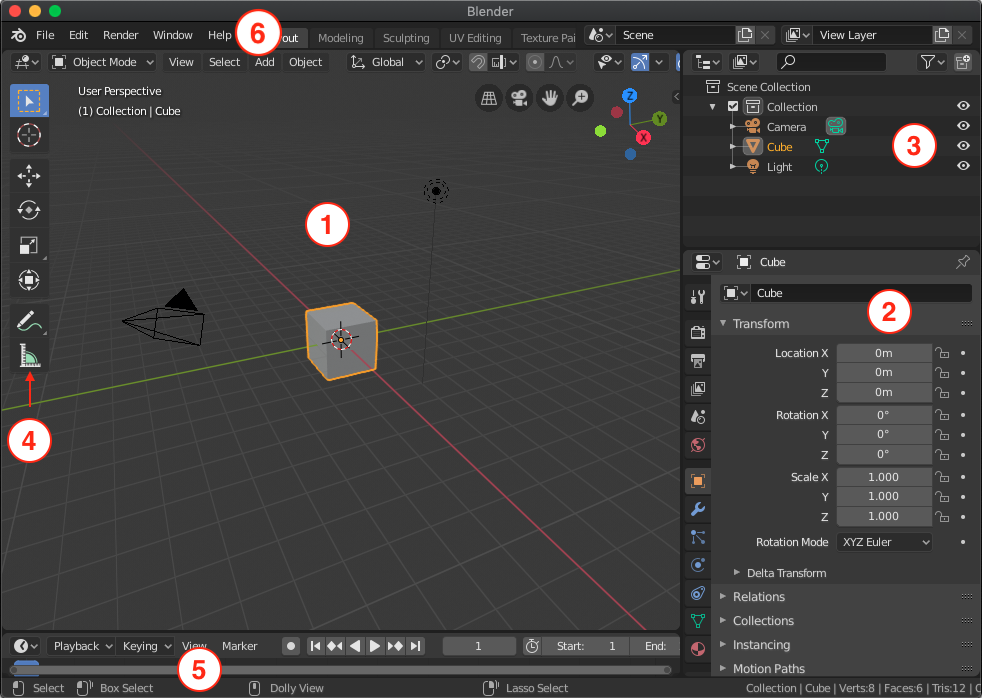
\includegraphics[width=1.0\textwidth]{blender-interface}
}

\noindent This is the default configuration of Blender when you open it for the first time.  Each
panel that you see in the above screenshot is labeled as follows:
\begin{enumerate}
    \item The \textbf{3D View} is your main view into the scene you are editing.  Unsurprisingly,
    this is where most of your work happens.  We will talk more about how to navigate the 3D view
    in the subsection below.  This is similar to the scene view in Unity.
    \item The \textbf{Properties} panel allows you to edit various properties of your scene, 
    including the camera, the currently selected object, the currently selected mesh, textures,
    materials, and so on.  We will often use the Properties panel throughout this tutorial.
    The Properties are analogous to Unity's inspector.
    \item The \textbf{Outliner} lists all of the objects, meshes, armatures (we'll get to this in a
    later lecture), and so on in your scene.  The outliner is most similar to the hierarchy view in
    Unity.
    \item The \textbf{Tool Shelf} contains shortcuts for common editing operations.  You can toggle
    the tool shelf on and off with \keys{T}.  If you ever forget a shortcut, the tool shelf is your
    friend!
    \item The \textbf{Timeline} is used to scrub through animations (we will talk about 3D animation
    in a later lecture).
    \item The \textbf{Info} panel contains common menus like \menu{File} and \menu{Window}, and
    allows you to change between preset layouts.  If you ever want to reset the blender UI, use the
    dropdown: 
\includegraphics[height=1.0em]{layout-default} and select ``Default''.
\end{enumerate}

\begin{wrapfigure}{r}[30pt]{0.17\textwidth}
    \vspace*{-2em}
    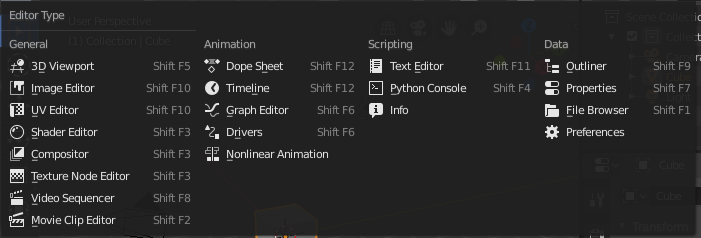
\includegraphics[width=0.17\textwidth]{editor-type-dropdown}
\end{wrapfigure}
You may have noticed that at the corner of each panel there is a dropdown.  This dropdown allows
you to change the \textit{Editor Type} of each panel.  For example, we can change from the 3D view 
to the text editor by clicking on the dropdown on the bottom left of the 3D view and selecting ``Text 
Editor.''  Fun fact: the entire blender front-end is written in python and is fully scriptable and
extendable.  The text editor is used to write python scripts for blender -- but we won't be using it
now.  Switch back to the ``3D View'' using the same dropdown.  Also notice how all of the panels
discussed on the last page are available here.  For example, it may not be all that useful, but you 
can change the 3D view into a huge timeline.

You can resize each panel by clicking and dragging at the borders.  If you want to create more editor
views than the default, \textbf{right click} on the border of two panels and select \menu{Split Area}.
Then move your mouse over the panel you would like to split and \textbf{left click} to apply.  This
process is detailed below:

{
\centering
\begin{minipage}{0.15\textwidth}
    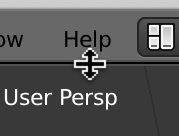
\includegraphics[width=1.0\textwidth]{split-1}\\
    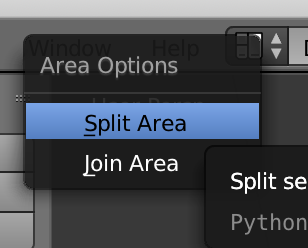
\includegraphics[width=1.0\textwidth]{split-2}
\end{minipage} $\rightarrow$
\raisebox{-.45\height}{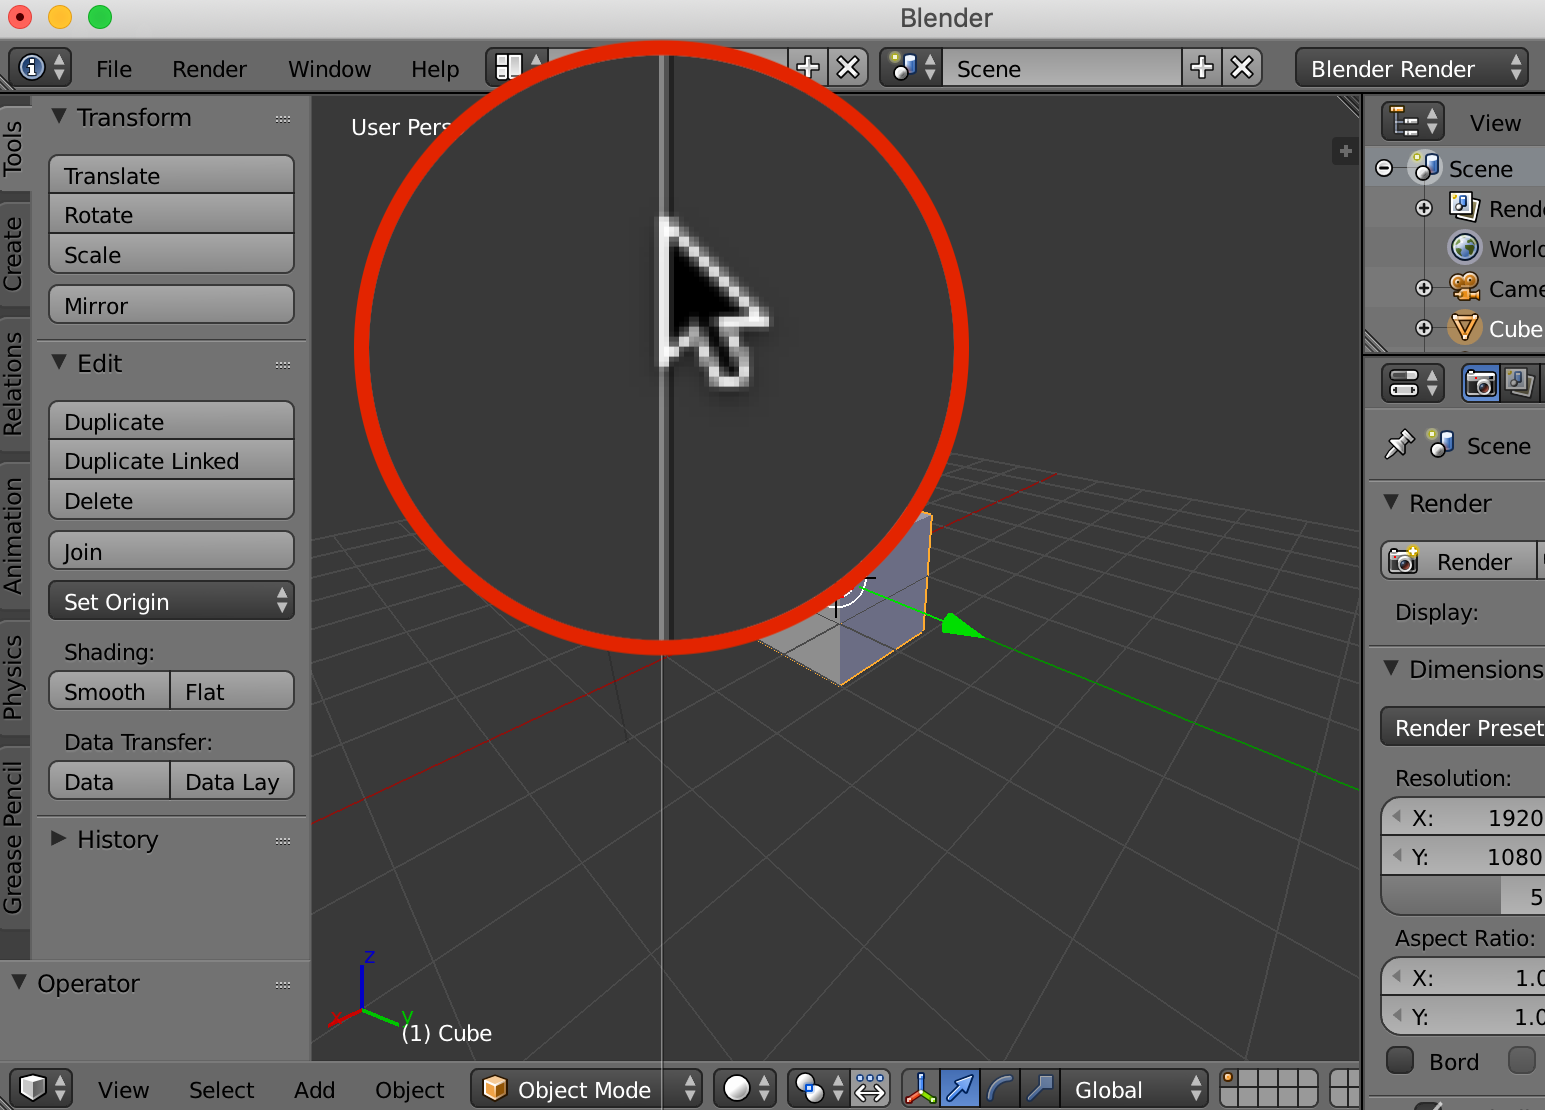
\includegraphics[width=0.36\textwidth]{split-3}} $\rightarrow$
\raisebox{-.45\height}{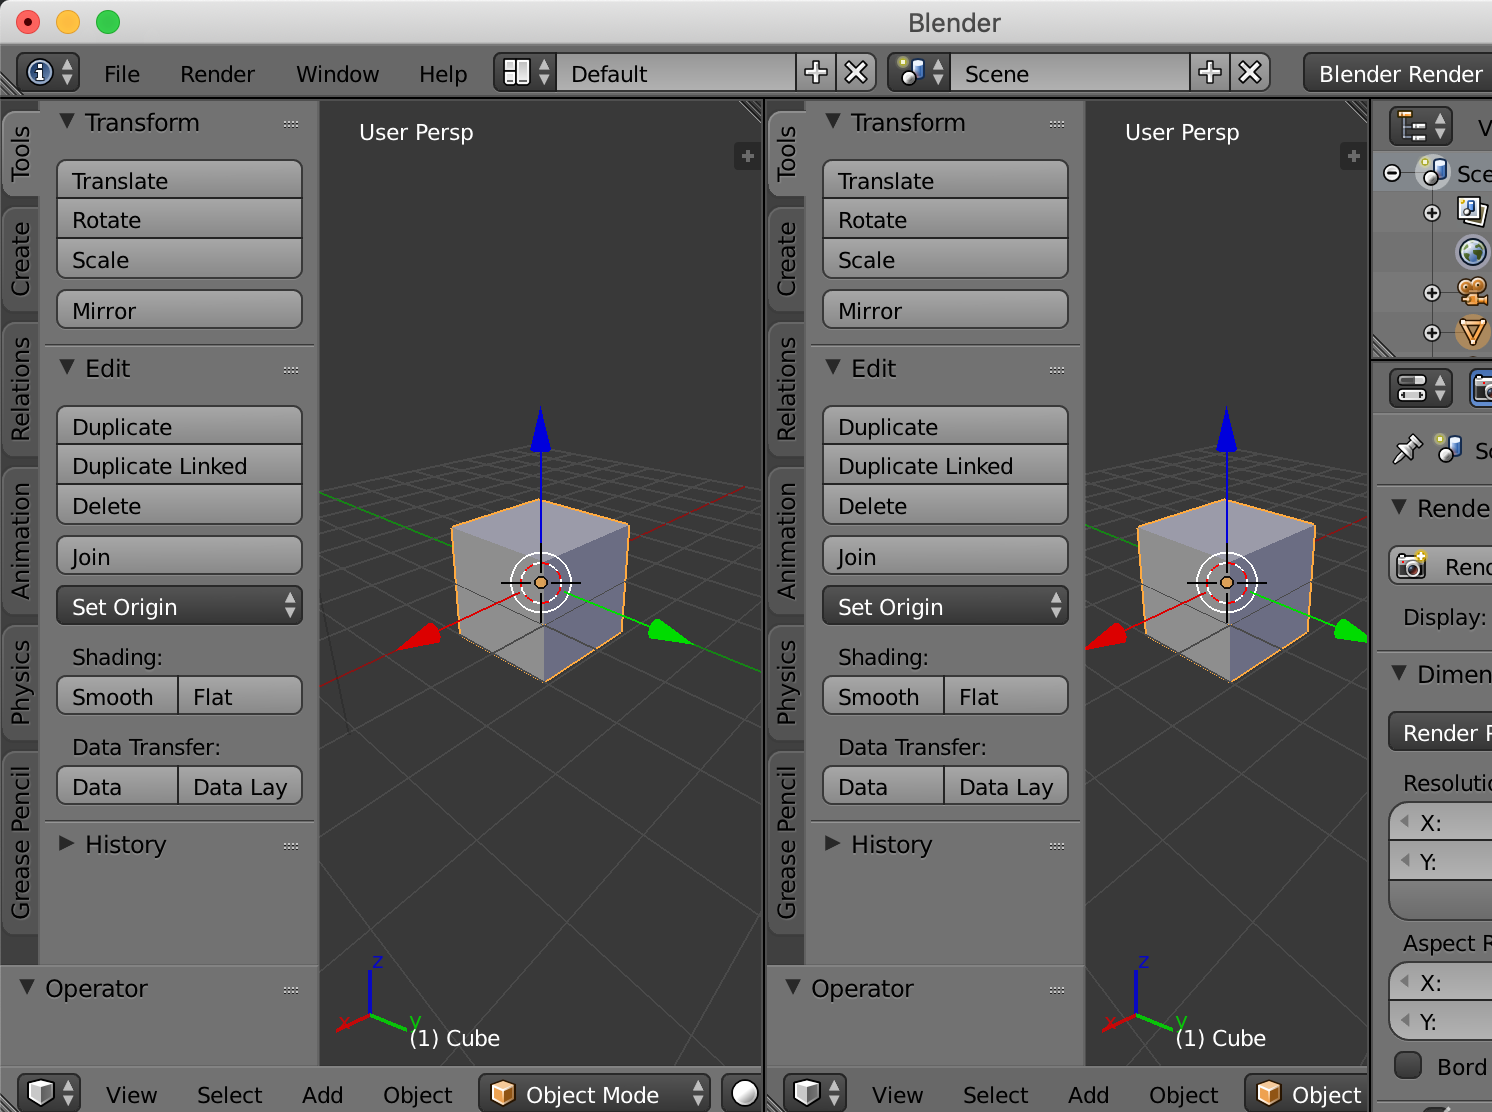
\includegraphics[width=0.36\textwidth]{split-4}}
\vspace{0.7em}
}

\noindent You can also select ``Join Area'' and click on one of the two bordering panels to join
them together.

\subsection{Navigating the 3D View}

You can navigate the 3D view using the following controls:
\begin{itemize}
    \item To \textbf{orbit} (rotate) the view, hold \keys{Middle Mouse Button} while dragging the
    mouse.
    \item To \textbf{pan} (translate) the view, hold \keys{Shift+Middle Mouse Button} while dragging
    the mouse.  You can also hold \keys{Shift+Ctrl+Midle Mouse Button} to ``Dolly Zoom'', which
    moves the camera forward and backwards.
    \item To \textbf{zoom} the view, hold \keys{Ctrl+Middle Mouse Button} while dragging the mouse,
    or scroll \keys{Mouse Wheel}.  This is different than the dolly zoom because the viewport camera
    does not move.
    \item If you ever get lost, press \keys{Numpad {\Large.}} (period) to zoom and pan to the 
    currently selected object.
\end{itemize}

\subsection{Working in Object Mode}

\begin{wrapfigure}[4]{r}[30pt]{0.3\textwidth}
    \centering \vspace*{-3.5em}
    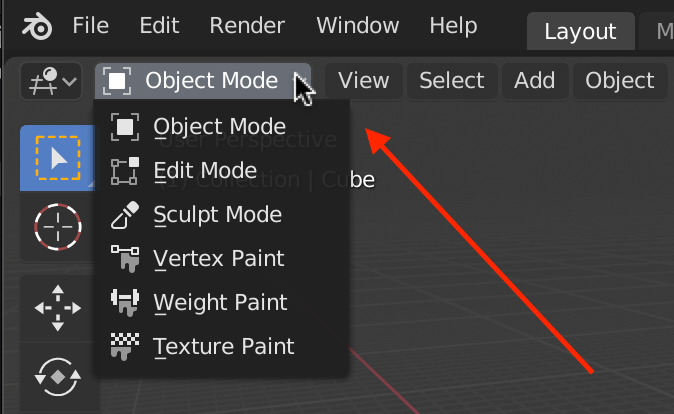
\includegraphics[width=0.3\textwidth]{mode-switcher}
    The Mode Switcher
\end{wrapfigure}
By default, when blender opens you will be in \textbf{Object Mode}.  You can verify what mode you 
are in by checking the \textit{Mode Switcher} at the bottom of the 3D View.  Each \textbf{Object} in blender
(analogous to a GameObject in Unity terminology) has a \textbf{Mesh} attached.  Just like in Unity,
you can transform Objects.  Below are some common shortcuts to manipulate objects in Object Mode 
(\textit{Important: Make sure your mouse is on top of the 3D view when using these shortcuts, because
shortcuts are different depending on which view is ``active.''})

\begin{itemize}
    \item Press \keys{Right Mouse Button} to select an object.  \textbf{Important: Left Mouse button
    does not select objects in blender!}  This is a common point of confusion for new users.
    \footnote{I know this is really confusing,  but there is hope: in the Blender 2.8 beta, the 
    developers have changed the default to left-click select.  As you can imagine, this has been a
    source of debate and nerd wars in the blender community for \textit{decades}!}
    \item Press \keys{Left Mouse Button} to move the \textit{3D cursor}.  The 3D cursor is used for
    many 3D operations as a reference point -- for now, though, you can largely ignore it.
    \item Press \keys{G} (``Grab'') to Move an object, \keys{R} (``Rotate'') to Rotate an object,
    or \keys{S} (``Scale'') to Scale an object.  You can move the mouse to control the 
    transformation; click \keys{Left Mouse Button} or press \keys{\return} to apply.  While grabbing
    / rotating / scaling, you can press \keys{X} / \keys{Y} / \keys{Z} to constrain the 
    transformation to a single axis.  Press the same key again to switch from Global axes (relative
    to the origin) to Local axes (relative to how that object is rotated).  Also, if you press
    \keys{Shift+X}, you will constrain the transformation to every axis \textit{except for} the X
    axis--this is useful if you want to move an object along another face.
    \item Alternatively, you can use the on-screen 3D manipulators to move objects.  You can change
    the type of manipulator on screen by using the selector 
    (\raisebox{-0.25\height}{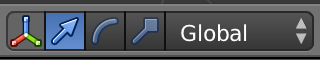
\includegraphics[height=1.5em]{manipulator-type-switcher}}) located at the bottom of the 3D View.  You can also use the pivot switcher
    (\raisebox{-0.25\height}{
\includegraphics[height=1.5em]{pivot-switcher}}) to change the pivot
    point of any transformation.  One useful feature is the ability to change the pivot to the 3D
    cursor.  This allows you to (for example) rotate an object \textit{about} the 3D cursor
    \item Press \keys{X} to delete an object.
    \item Press \keys{Shift+D} to duplicate an object.  You can also press \keys{Alt+D} to 
    ``Duplicate Linked,'' which shares the same mesh between the two objects.  This is similar to
    the idea of prefabs in Unity: editing the mesh of either object will affect the appearance of
    both.  This is especially useful because this link will actually persist when you import to
    Unity -- cool!
    \item Press \keys{B} to box-select and \keys{C} to circle-select objects.
    \item Press \keys{T} to toggle on and off the Toolshelf.  The toolshelf has clickable buttons
    for many common editing operations (including all of the shortcuts listed above).
    \item Press \keys{N} to toggle on and off the \textbf{Properties} panel.  The properties panel
    allows you to directly manipulate the position / rotation / scale of whatever you have selected,
    as well as various miscellaneous settings for how the mesh displays in the 3D View.
    \item Press \keys{A} to select all or deselect all (depending on if anything is selected).
\end{itemize}

Blender has an incredibly robust shortcut system -- almost \textit{every} common editing operation
has a corresponding shortcut.  So while it may be difficult to get used to blender's UI, mastery of
it will allow you to do things very quickly.  For example, rotating an object 45 degrees in
the Z axis is as easy as \\\keys{R} \faAngleRight\ \keys{Z} \faAngleRight\ \keys{4} \faAngleRight\ 
\keys{5} \faAngleRight\ \keys{\return}.  That being said, it is still very easy to forget all of the random 
incantations--er--key combinations you need to use to do what you want.  Luckily, pressing \keys{Space} at
any time will bring up a search bar that allows you to search for any operation.  It will also show any
relevant key combinations.  You can then hit \keys{\return} to apply the operation.
\begin{center}
    \vbox{
    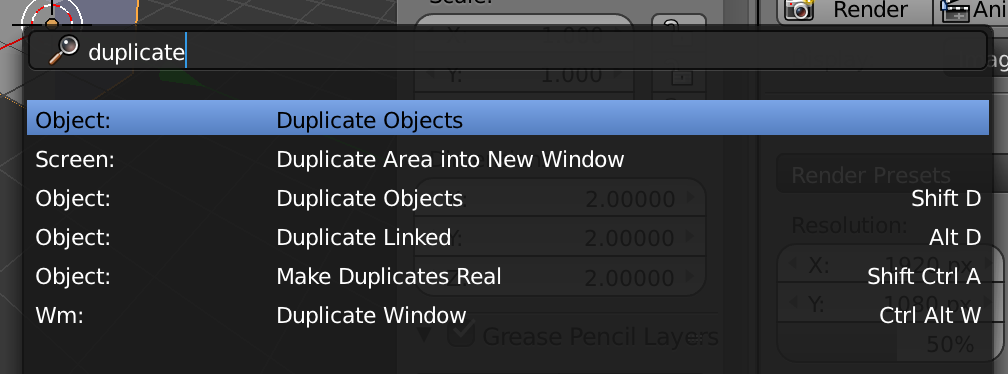
\includegraphics[width=0.5\textwidth]{search-diag}\\
    Searching for Shortcuts}
\end{center}

\subsection{Creating Objects}

You can create new blender objects via the \menu{Add>Mesh} menu at the bottom of the 3D View.  There
are plenty of other types of objects in the \menu{Add} menu, but since we are creating a video game
we have to use polygonal meshes that can be imported to Unity.  If you were, for example, interested
in making a film, or if you wanted to create a very high-detail model that will be later converted
a game-ready mesh, you may want to look into the other surface types.  Check out the 
\href{https://docs.blender.org/manual/en/latest/modeling/index.html}{Blender Manual} for more info!
Also, as always if you don't want to trawl through menus you can use ex \keys{Space+``Add Cube''+\return}
to add a cube to the scene.  Note that new objects will be placed at the \textit{3D cursor} location.
If you can't find your 3D cursor, you can change its location in the Properties panel (\keys{N}).

\subsection{Parenting Objects}

Just like in Unity, you can parent two objects to each other in blender.  Any transformations done
to the parent will ``trickle down'' to the children in an hierarchical fashion.  You can parent
objects in two ways:
\begin{enumerate}
    \item In the outliner, \textbf{left click and drag} on the \textbf{icon} to the left of one 
          object, and drag the icon on top of another object
    \item Select the child object(s), then the parent, and press \keys{Ctrl+P}.
\end{enumerate}
Conveniently, parented objects will import to Unity with the same relative transformations.

\section{Local Mesh Editing}

Well it's been \thepage\ pages and we haven't even started modeling yet--blender is a pretty complex
piece of software!  Luckily, the UI is consistent (albeit complex) so editing meshes is very similar
to editing objects.  To edit an object's mesh, select it and switch to \textbf{Edit Mode}.  The
shortcut to switch between Object and Edit Mode is \keys{Tab}.  You can also use the Mode Switcher
(mentioned above in ``Working in Obect Mode'') to switch to Edit Mode.  That being said, you will
be switching between Object/Edit so often that \keys{Tab} is worth memorizing.  \textit{Important:
make sure you have an object selected or you can not go into Edit Mode.}

You'll notice a few things when switching from Object to Edit mode.  First, the individual vertices
of the mesh will be selected.  A \textbf{vertex} (plural \textit{vertices}) is an individual point
on the mesh.  Vertices are connected by \textbf{edges}, and edges are connected by \textbf{faces}.
You can select vertices with \keys{Right Mouse Button}, just like how you selected objects before.
In addition to this, the tools at the Bottom of the 3D view as well as the Toolbar / Properties
panels update according to the current mode.  It's important to be aware of what mode you're in so
that you don't get disoriented with the UI.

At the bottom of the 3D view, click on the buttons that look like this:  
\raisebox{-0.25\height}{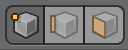
\includegraphics[height=1.5em]{select-switcher}} to change between Vertex,
Edge, or Face selection.  As always, use \keys{Right Mouse Button} to select each type.  You can
hold \keys{Shift} to select multiple elements of your mesh.  Just like in object mode, you can
press \keys{G} / \keys{R} / \keys{S} to Move / Rotate / Scale parts of your mesh (see ``Working in
Object Mode'' above).  More complex operations can be accessed via the \menu{Mesh > Vertices},
\menu{Mesh > Edges}, or \menu{Mesh > Faces} menus.  The shortcut for these are \keys{Ctrl+V},
\keys{Ctrl+E}, and \keys{Ctrl+F} respectively.  There are lots of very useful features in each of
these menus (and other submenus), but I will cover the most common / useful below.

\begin{itemize}
    \item \textbf{Extrude} (Shortcut \keys{E}): Takes whatever you have selected, duplicates it, and
    connects what you selected to the duplicate.  For convenience, transitions into grab mode, as if
    you pressed \keys{G}, so that you can move the extruded object.  This has slightly different
    implications depending on if you selected a Vertex, Edge, or Face (see below pictures, respectively):\\
    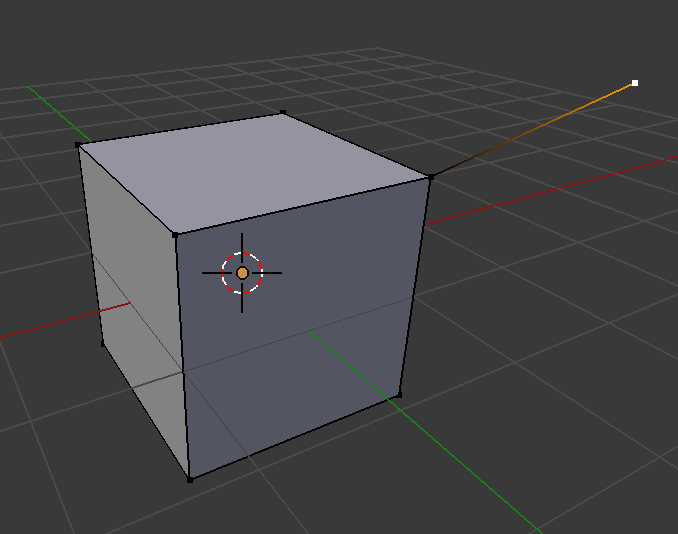
\includegraphics[height=10em]{extrude-vertex} 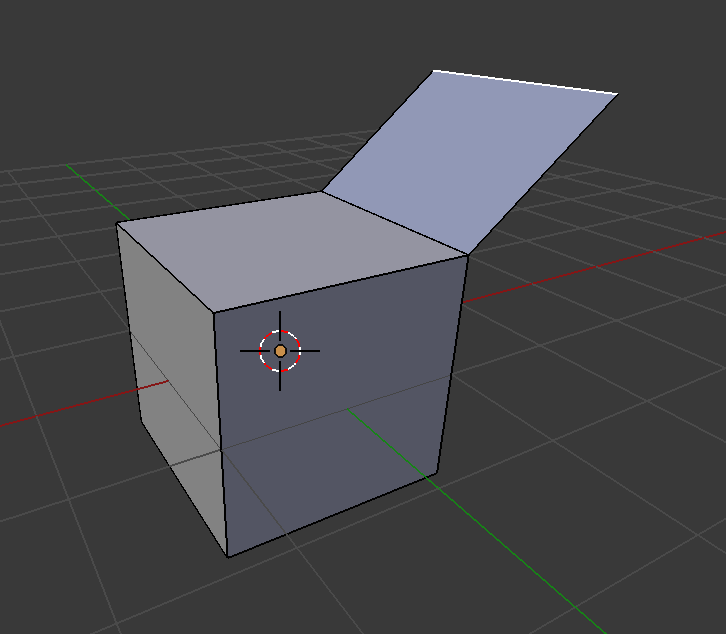
\includegraphics[height=10em]{extrude-edge}
    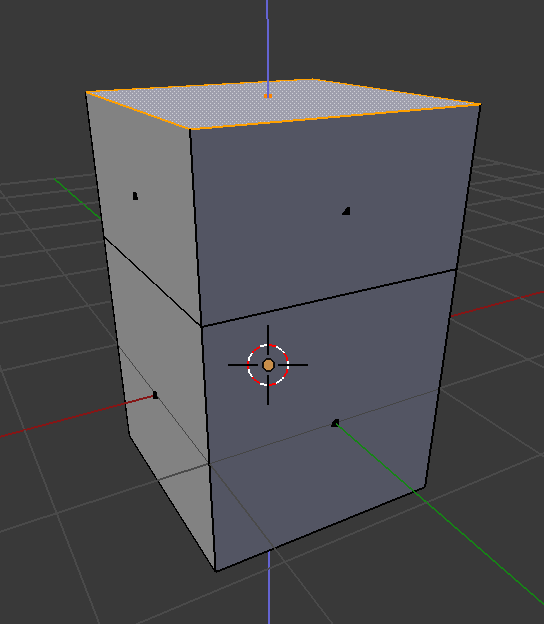
\includegraphics[height=10em]{extrude-face}
    \item \textbf{Delete} (Shortcut \keys{X}): Deletes a vertex, edge, or face.  When you press
    \keys{X}, a menu will appear with many different options for what exactly you want to delete,
    and how.  For example, selecting \menu{Vertices} will delete all selected vertices (and all
    connected geometry), but \menu{Faces} will only delete the selected faces without modifying
    connected geometry: \\
    \raisebox{-.45\height}{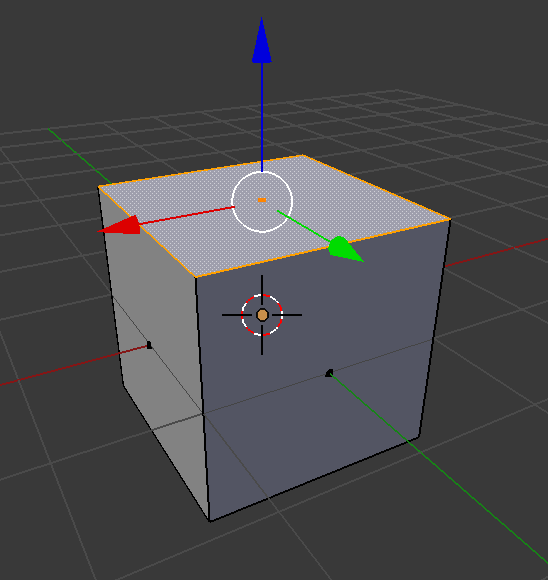
\includegraphics[height=10em]{delete-1}} $\rightarrow$
    \raisebox{-.45\height}{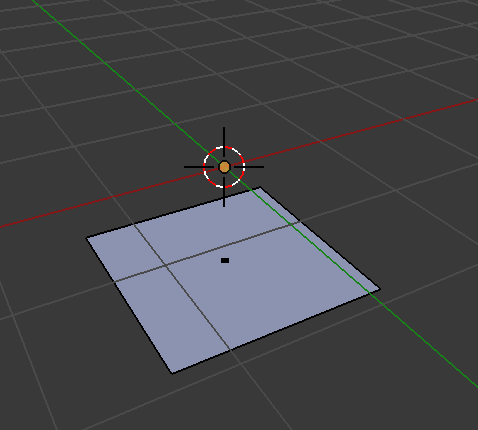
\includegraphics[height=10em]{delete-2}}
    \ /\ \raisebox{-.45\height}{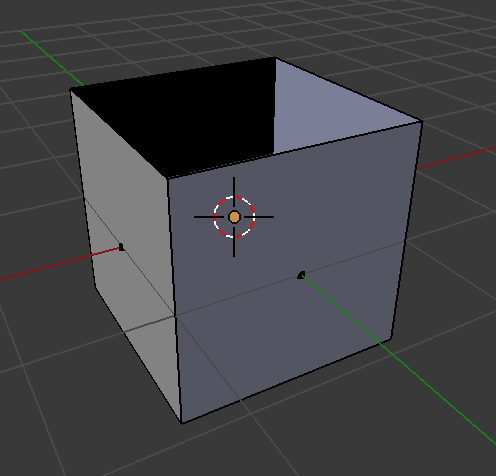
\includegraphics[height=10em]{delete-3}}\\
    \vbox{\item \textbf{Subdivide} (Shortcut \keys{W}, then click \menu{Subdivide}): This command divides
    a face or edge into equal sections:\\
    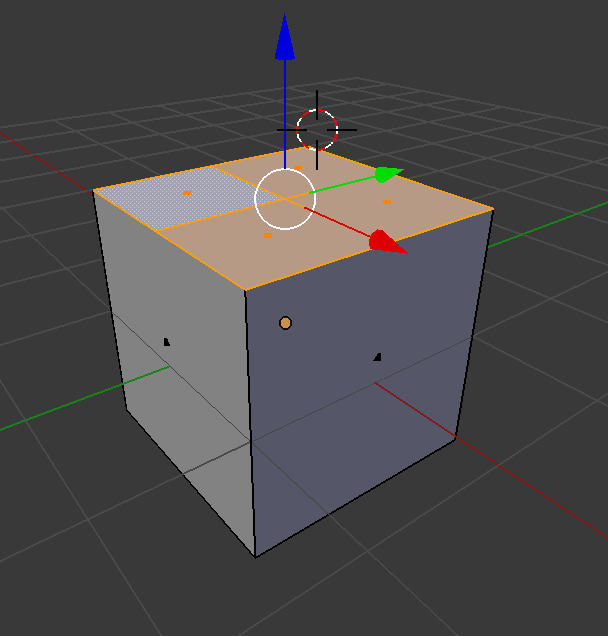
\includegraphics[height=10em]{subdivide-face} 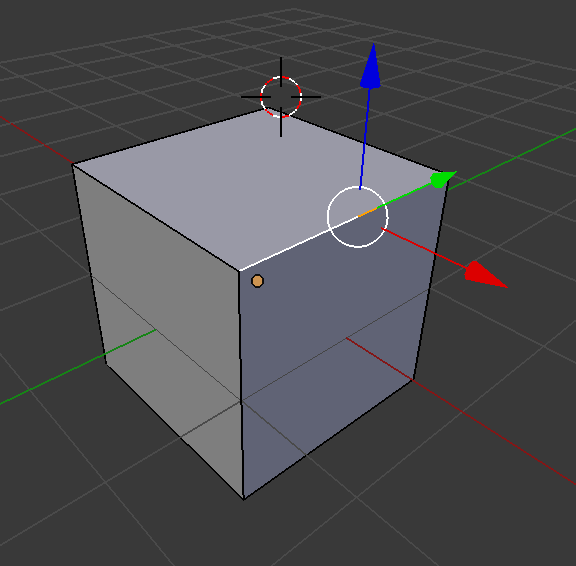
\includegraphics[height=10em]{subdivide-edge}}
    \item \textbf{Merge} (Shortcut \keys{W}, then click \menu{Merge...}, OR \keys{Alt+M}): Merges
    all selected vertices, edges, or faces into a single vertex.  If you are selecting vertices,
    you have a lot of control as to where the merged vertex ends up (for example, you can set it
    to merge to the center of all points you selected to merge, or you can set it to merge to the
    first or last point you selected, etc).
    \item \textbf{Snap} (Shortcut \keys{Shift+S}) will snap the current selection to the cursor,
    other selected objects, or \textit{the grid}.  The snapping grid is useful to keep your selection
    on a uniform grid -- you can modify the size of the snapping in the \menu{Display>Grid Scale} submenu of
    Properties (shortcut \keys{N}).  You can also snap all transformations to the grid via the
    snap button (
\includegraphics[height=1.5em]{snap-settings}) at the bottom of the 3D View.
    You can also use \keys{Shift+S} to snap the 3D cursor to things--notably, you can snap the 3D
    cursor to the origin, which is a fast way to reset the 3D cursor position when you left click
    by accident \faMehO
    \item \textbf{Loop Cut} (Shortcut \keys{Ctrl+R}) will create a ring around the mesh.  Using
    loop cuts to create new vertices is highly recommended as it maintains good topology of the mesh
    (you generally want to avoid triangles, especially very obtuse ones as they animate badly).
    \item \textbf{Select Edge Loop} (\keys{Alt+Right Mouse Button} while hovering an edge) selects 
    all the edges that are in a contiguous loop.  This is useful in many situations, for example you
    could select all of the edges around a character's torso.
    \item \textbf{Knife Cut} (Shortcut \keys{K}) will allow you to simply cut through the mesh using
    the mouse.
    \item \textbf{Vertex Slide} (Shortcut \keys{G} \keys{G} in Vertex select mode) slides a vertex
    along one of its edges.
    \item \textbf{Wireframe Mode} (Shortcut \keys{Z}) allows you to see through the mesh and select
    vertices / edges / faces that are behind other faces.\\
    \vbox{\item \textbf{Proportional Editing} (Shortcut \keys{O}) allows you to ``pull'' a neighborhood
    of Vertices / Edges / Faces in a weighted way, based on a falloff distance from what you have
    selected.  You can change the falloff settings at the bottom of the 3D View (
    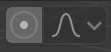
\includegraphics[height=1.5em]{propedit-1} / 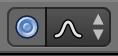
\includegraphics[height=1.5em]{propedit-2} when
    enabled); open the dropdown to change the falloff type.  You can change the falloff distance
    with \keys{Mouse Scroll Wheel}:\\
    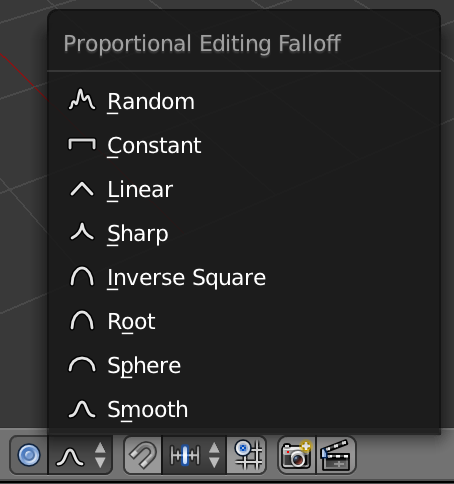
\includegraphics[height=10em]{propedit-3} 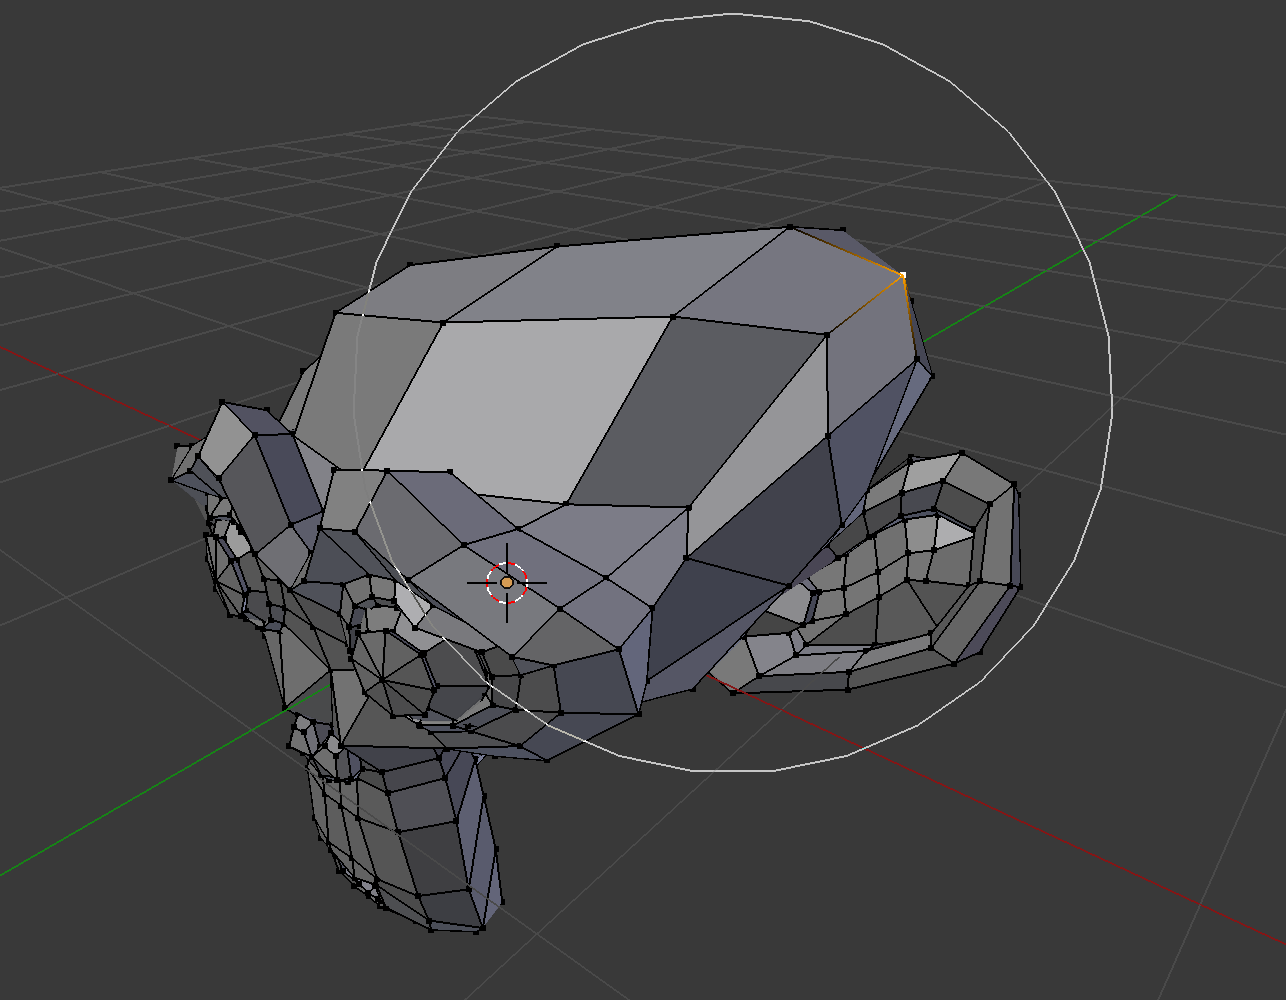
\includegraphics[height=10em]{propedit-4}}\\
    Proportional editing applies to Move, Rotate, and Scale operations in Vertex, Edge, or Face
    select.
\end{itemize}

\section{Using Modifiers for Global Editing Operations}

The operations that we have talked about so far are \textit{Local Operations}.  This means that they
only affect the Faces, Edges, or Vertices that you specifically select.  However, oftentimes you
want to perform \textit{Global Operations} on the entire mesh.  The easiest way to perform ``object-
wide'' operations on meshes is to use \textbf{Modifiers}.  Modifiers can be accessed from the
Properties panel when you have an object selected.  \textit{Note: you must switch to Object Mode
before adding Modifiers to your mesh.  If you don't you may not see the results of applying the
modifier until you switch out to Object mode.}

As a test, I'll add in the \menu{Monkey} primitive (\menu{Add>Mesh>Monkey}), which is useful as a
semi-complex object to play with.  Her name is \textit{Suzanne}, and she is
the official mascot of Blender.  \footnote{Why a monkey?  Suzanne is one of a few very popular 
\href{https://en.wikipedia.org/wiki/List_of_common_3D_test_models}{Test Models}, alongside the
``Stanford Bunny'' and the ``Utah Teapot,'' which you'll tend to see in many Computer Graphics
research papers.}  Open up the Modifiers tab in the Properties panel.  You can click ``Add 
Modifier'' to add a new modifier to the object:
\begin{center}
    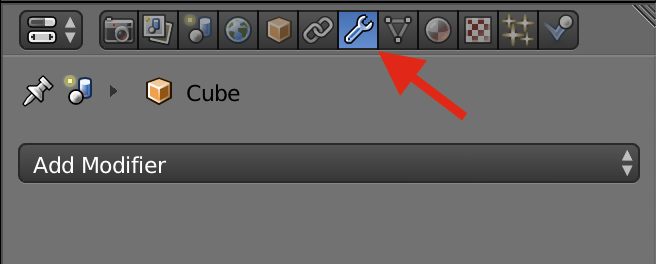
\includegraphics[width=0.4\textwidth]{modifier-panel-1} 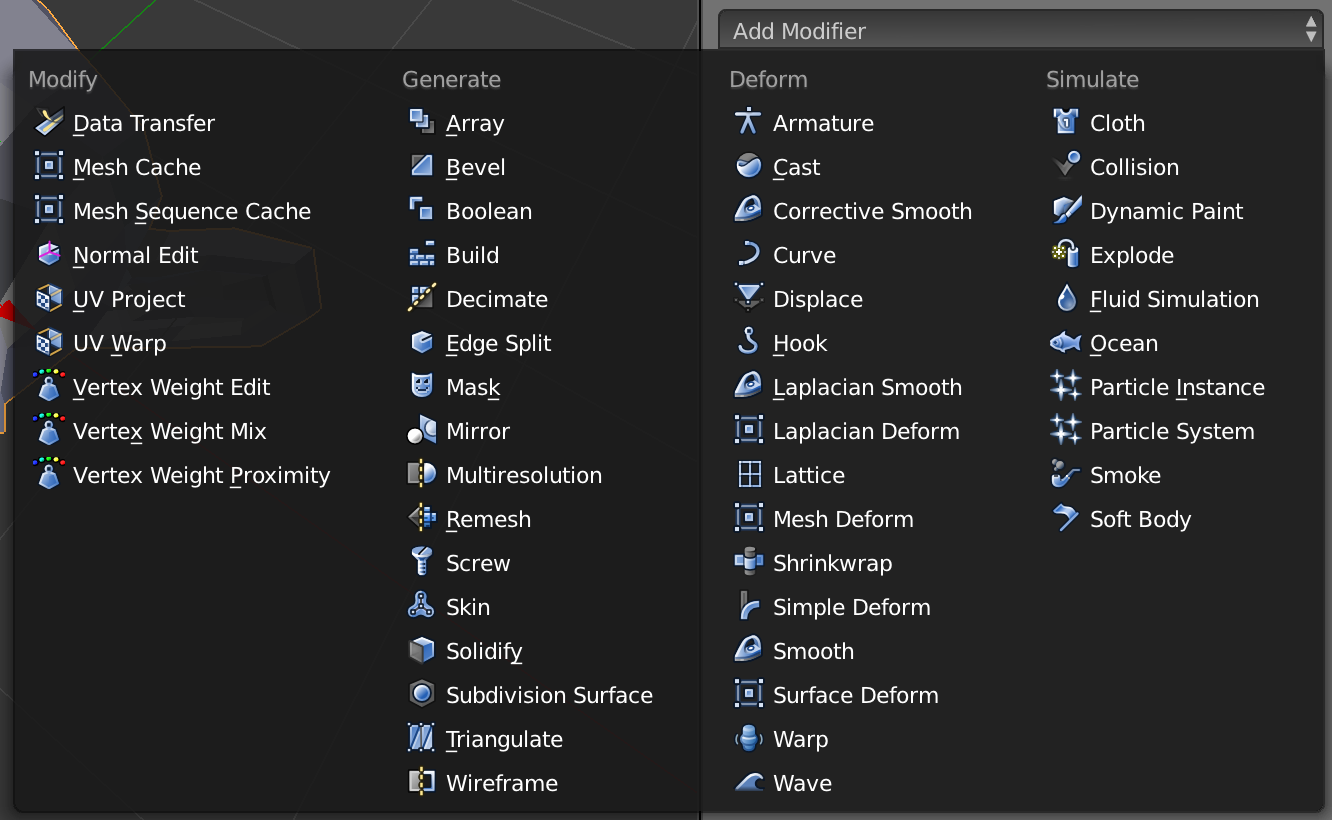
\includegraphics[width=0.4\textwidth]{modifier-panel-2}
\end{center}
I'll go through some of the most useful modifiers below.  You can find a more comprehensive 
reference of all of the modifiers in the 
\href{https://docs.blender.org/manual/en/latest/modeling/modifiers/index.html}{Blender manual}.

\subsection{Subdivision Surface Modifier}

The \textbf{Subdivision Surface} modifier subdivides every face in the entire mesh (see the
\menu{Subdivide} operation above) and computes a carefully-weighted average of them, resulting in a
much smoother version of the original mesh.  Change the \menu{View} parameter of the subdivision
surface modifier to increase the resolution.  Below is suzanne with and without the subdivision 
surface modifier applied.
\begin{center}
    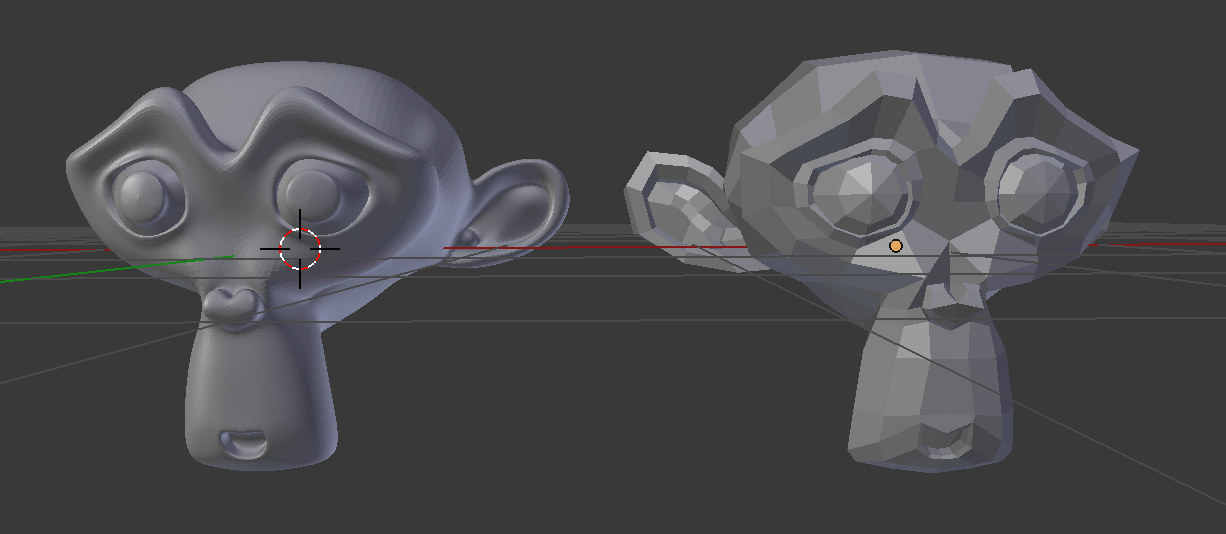
\includegraphics[height=10em]{subdiv-1} 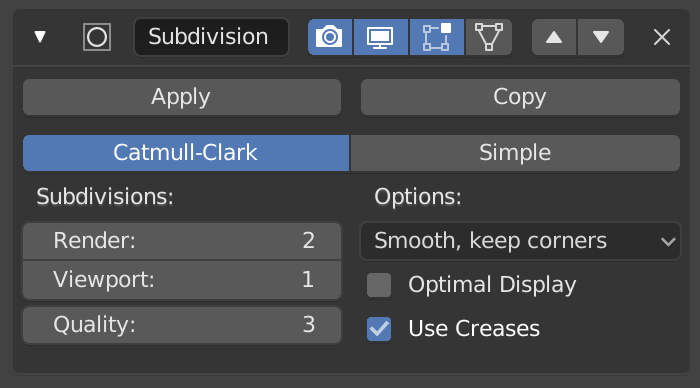
\includegraphics[height=10em]{subdiv-2}
\end{center}
You may recognize the algorithm name, ``Catmull-Clark,'' from Edwin Catmull, the President of Pixar.
In fact, Ed Catmull invented the algorithm along with Computer Scientist Jim Clark in 1978.  The
Catmull-Clark algorithm is what allowed early Pixar movies to represent complex smooth surfaces, and
was pivotal in creating convincing renderings of humans in their movies.  More info 
\href{https://en.wikipedia.org/wiki/Catmull–Clark_subdivision_surface}{here} on the algorithm.

\subsection{Mirror Modifier}
The \textbf{Mirror} modifier allows you to mirror a mesh along one of the principal (XYZ) axes.
This is useful if you want to edit a symmetrical mesh, such as a character.  Here I deleted half
of Suzanne using the box select tool (\keys{B}) and used the Mirror modifier to enable a symmetric
editing workflow:
\begin{center}
    \raisebox{-.45\height}{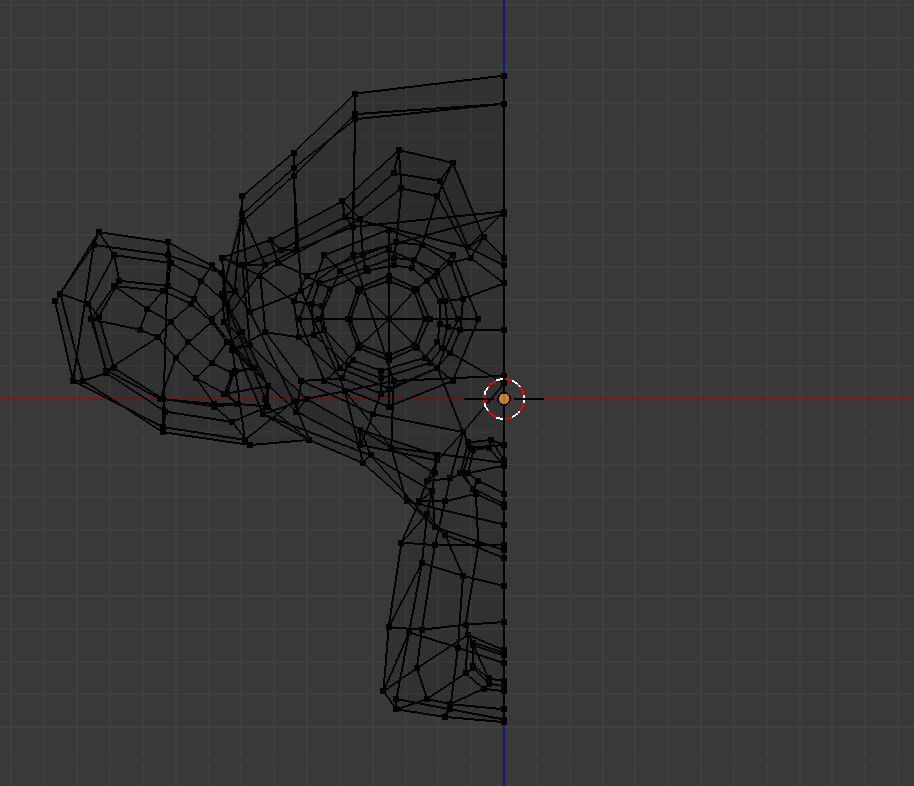
\includegraphics[height=10em]{mirror-1}} $\rightarrow$ 
    \raisebox{-.45\height}{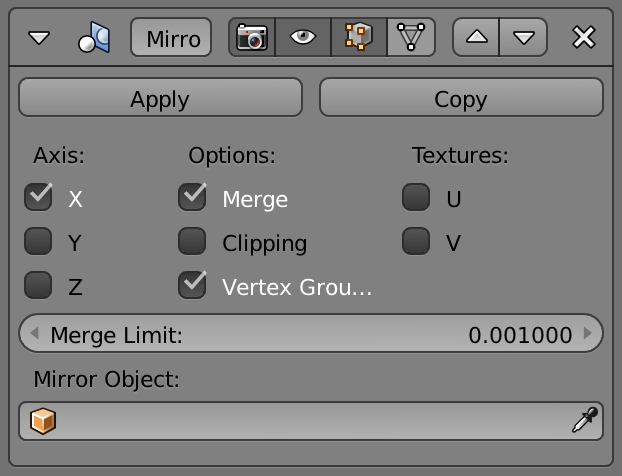
\includegraphics[height=10em]{mirror-2}} $\rightarrow$ \\
    \raisebox{-.45\height}{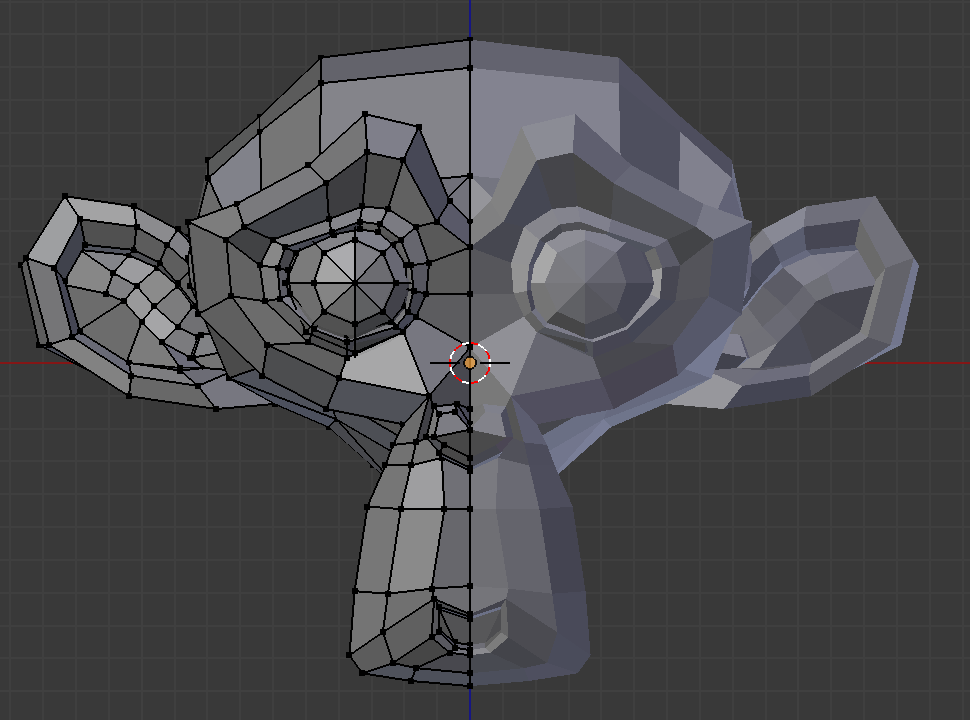
\includegraphics[height=10em]{mirror-3}} $\rightarrow$ 
    \raisebox{-.45\height}{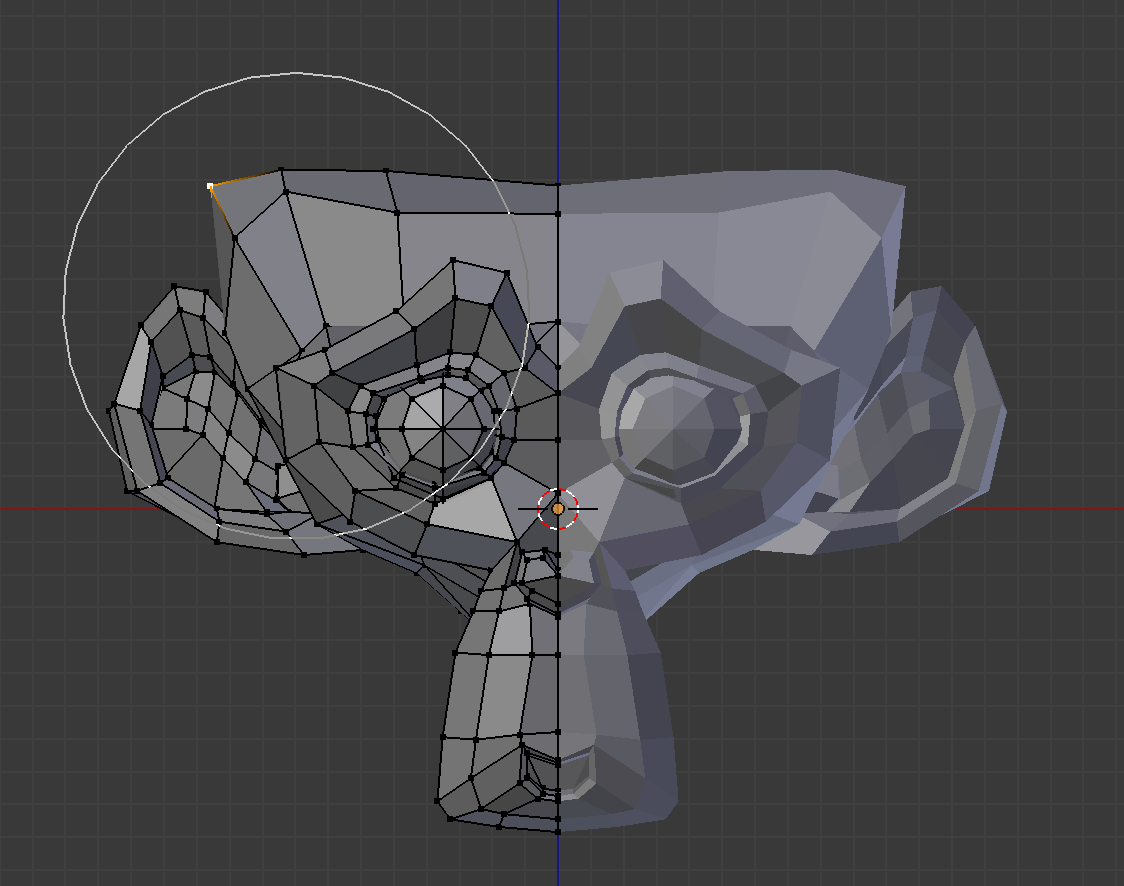
\includegraphics[height=10em]{mirror-4}}
\end{center}

\subsection{Nondestructive Editing}
A very useful feature of Modifiers is that they are \textbf{Nondestructive}.  For example, you can
edit the mesh after a mirror or subdivision surface modifier are added to an object, and the final
result will update as you would expect.  This is in contrast to simply performing the changes in
Edit mode, in which case the changes are permanent.  You can also click the \menu{Apply} button at
the top of every modifier to destructively apply it to the mesh.  This is useful if, for example,
you would like to tweak the output of a Subdivision Surface modifier, or if you would like to add
small asymmetric details to a character after blocking it out with the mirror modifier.

You can also add multiple modifiers to an object.  The modifiers are applied in the order that they
are added.  For example, you would want to apply a subdivision surface modifier \underline{after}
a mirror modifier.  Otherwise, you will get weird boundaries between the two halves:
\begin{center}
    \raisebox{-.45\height}{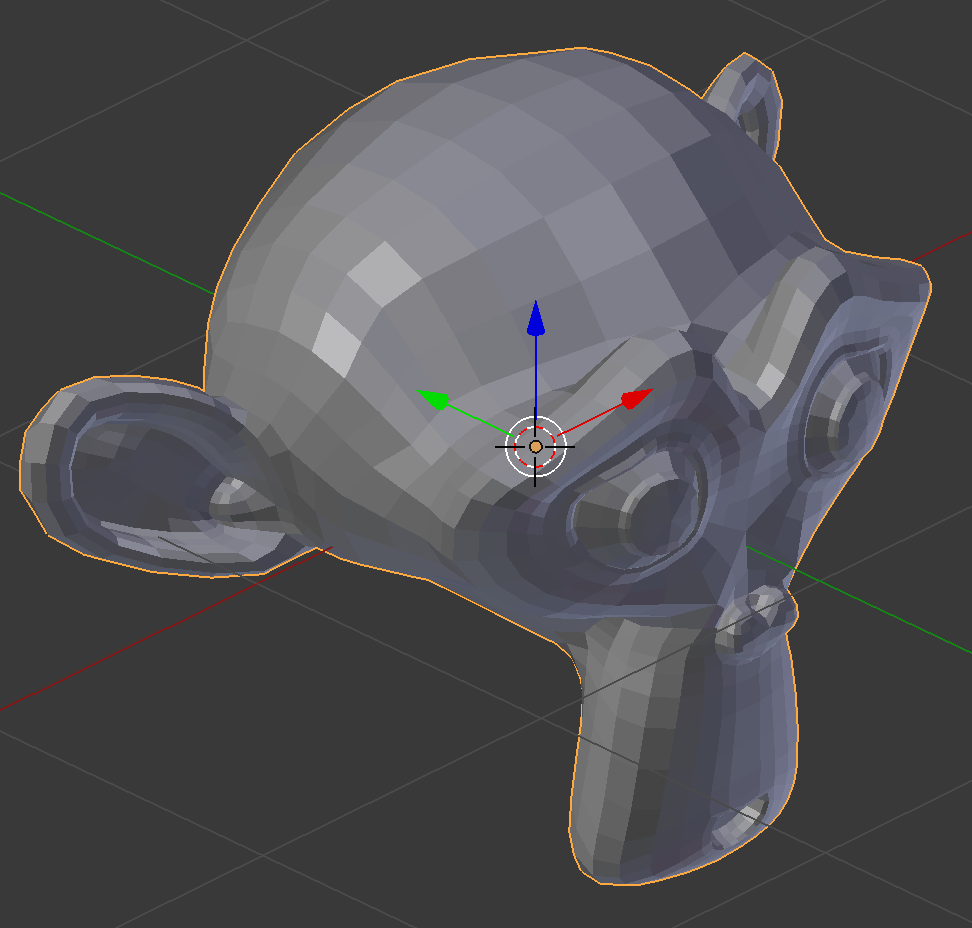
\includegraphics[height=13em]{nondest-1}} $\Big /$ 
    \raisebox{-.45\height}{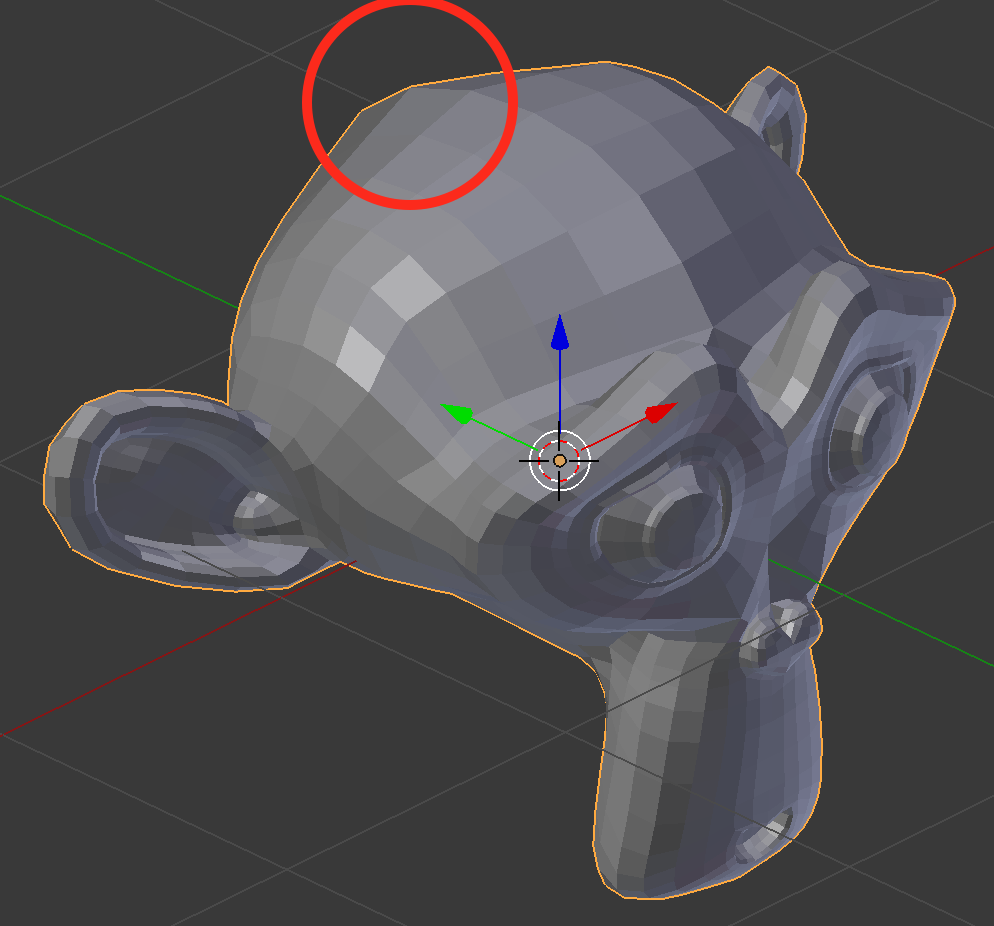
\includegraphics[height=13em]{nondest-2}} \\
    Left: Mirror First.  Right: Subdivision Surface First.
\end{center}
You can use the 
\includegraphics[height=1.5em]{modifier-stack-arrows} buttons at the top of each
modifier's UI to re-order modifiers.

\section{Texture Mapping}

Up to this point we have only talked about changing the shape or form of a 3D model.  What do we
do when we want to change the model's color?  Ideally, we want to be able to paint over the model
as if it were real-life clay model.  It would be great if we could use Photoshop for example to
define the model's color.  So how do we do this?  The solution is to use a technique called
\textbf{Texture Mapping}.  The essential idea is to create a \textbf{map} between an image file (a
``texture'') and your model.  In practice, this is done via something called a \textbf{UV Map}.
It's called a UV map because just like X, Y, and Z are used to describe the 3D axes in computer
graphics, we use U and V to describe the 2D axes on a texture.  It's just the common convention.

\begin{center}
    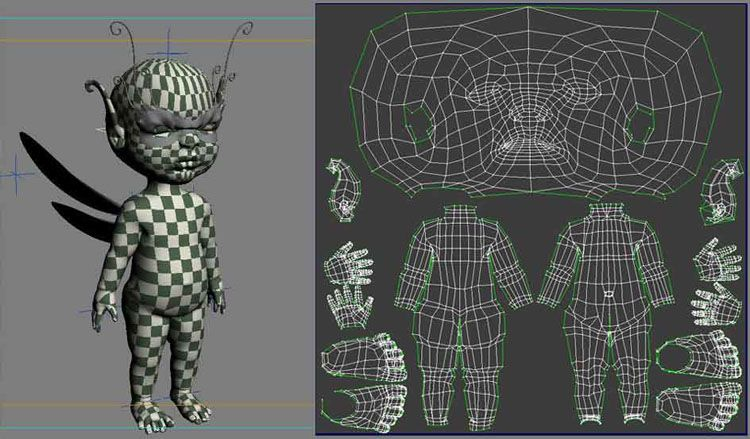
\includegraphics[height=15em]{uvmap} \\
    A UV map of a character \href{https://www.pinterest.com/pin/425730970997039889/}{(Source)}
\end{center}

You can think of a UV map as if you were wrapping the texture around your model, sort of like 
wrapping a present.  Or you could think about it in the inverse: how would we ``skin'' the model,
like skinning an animal's pelt, so that we could lay it flat?  We need to somehow tell Blender how 
to skin our model.  Let's walk through an example.

\subsection{UV Unwrapping a Campbell's Soup Can}

Let's create the textures and UV map for a simple model, a Campbell's Soup Can.  To begin, add a
Cylinder to the scene via \menu{Add>Mesh>Cylinder} in Object Mode.  We need to think about where we
would ``cut'' the model so that we could lay it out as flatly as possible on the UV map.  For a
cylinder, we would cut out the top and bottom circles, and then we would cut straight down the sides.
This would allow us to lay down the two circles and ``label'' flat next to each other with no 
stretching.  We can explicitly tell Blender to cut along specific edges using the \textbf{Mark Seam}
command.  You can get to this in edit mode via the edges menu (\keys{Ctrl+E}) then select 
\menu{Mark Seam}:
\begin{center}
    \raisebox{-.45\height}{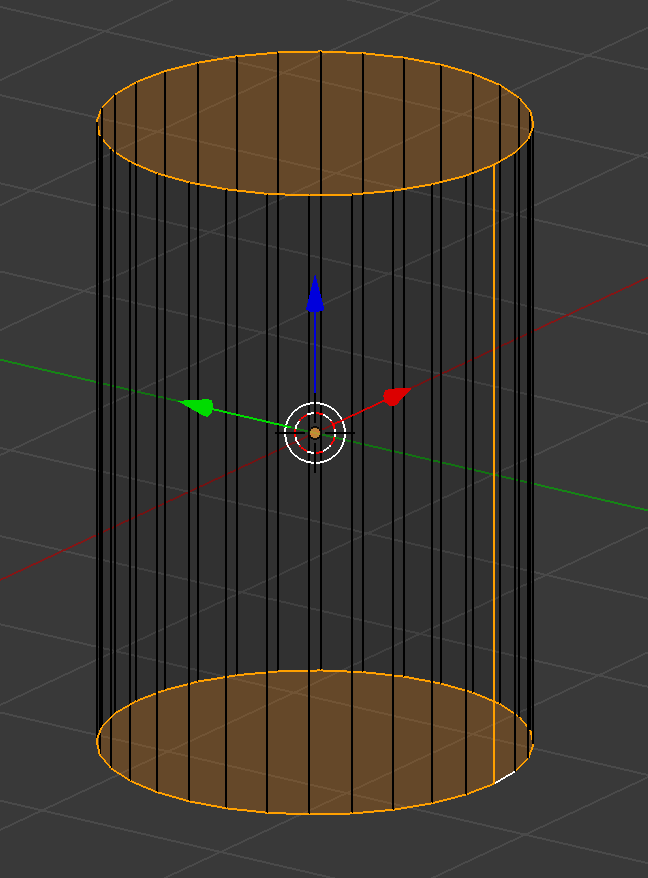
\includegraphics[height=10em]{seams-1}} $\rightarrow$
    \raisebox{-.45\height}{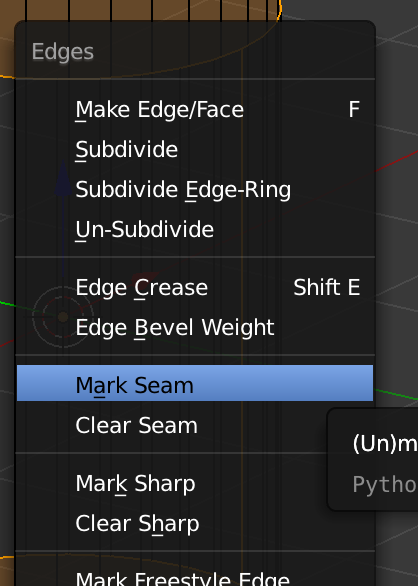
\includegraphics[height=10em]{seams-2}} $\rightarrow$
    \raisebox{-.45\height}{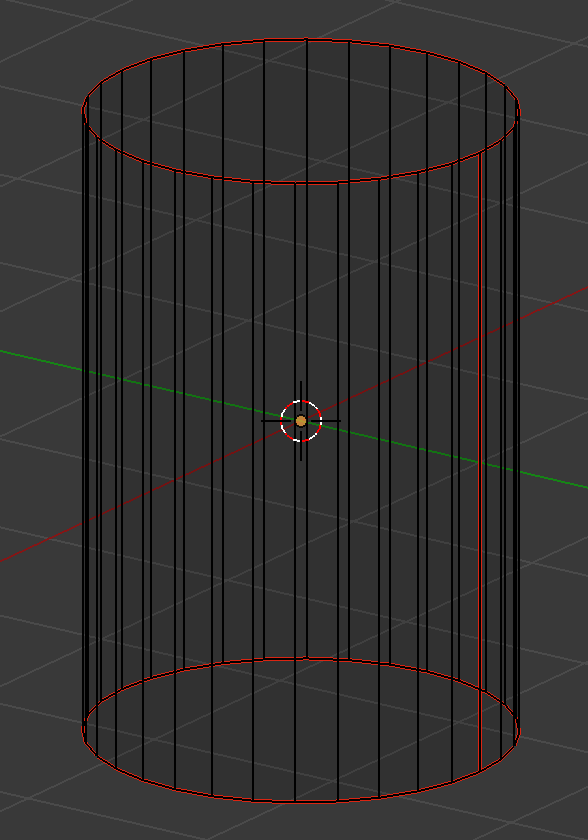
\includegraphics[height=10em]{seams-3}} \\
    Cutting up a Soup can with \menu{Mark Seam}
\end{center}
Next, we need to go ahead and create the UV Map.  First, create a new panel (see the section 
``Blender Interface Basics'' above) and open the \textbf{UV/Image Editor} View such that the 3D
View and the UV/Image Editor are placed side-by-side.  Recall that you can change the view of each
panel using the dropdown located in the corner of the panel.  Next, while hovering the mouse over
the 3D View in edit mode, press \keys{A} to select all, then open the \textbf{UV Mapping Menu}
with the \keys{U} key.  Select \menu{Unwrap}, and you should see our soup can fully unwrapped:
\begin{center}
    \raisebox{-.45\height}{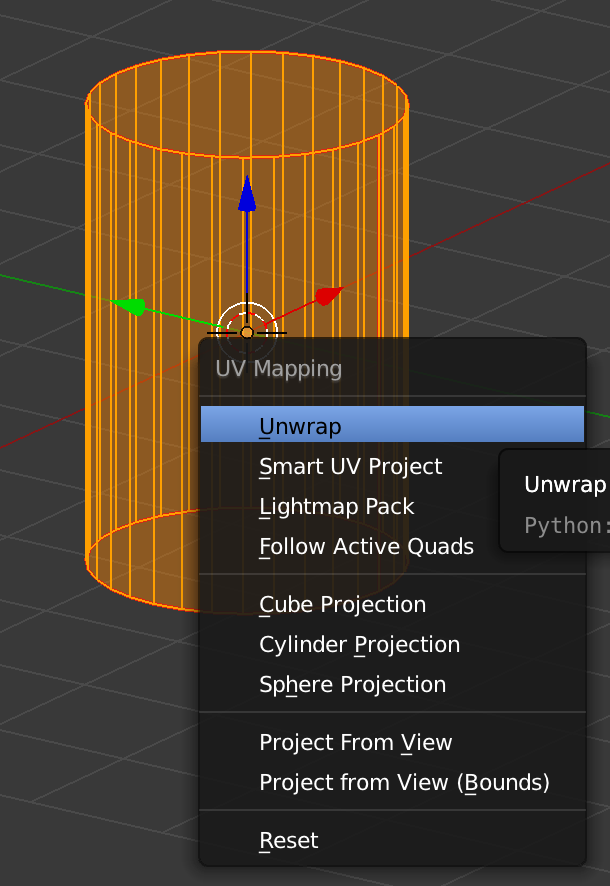
\includegraphics[height=15em]{unwrap-1}} $\rightarrow$
    \raisebox{-.45\height}{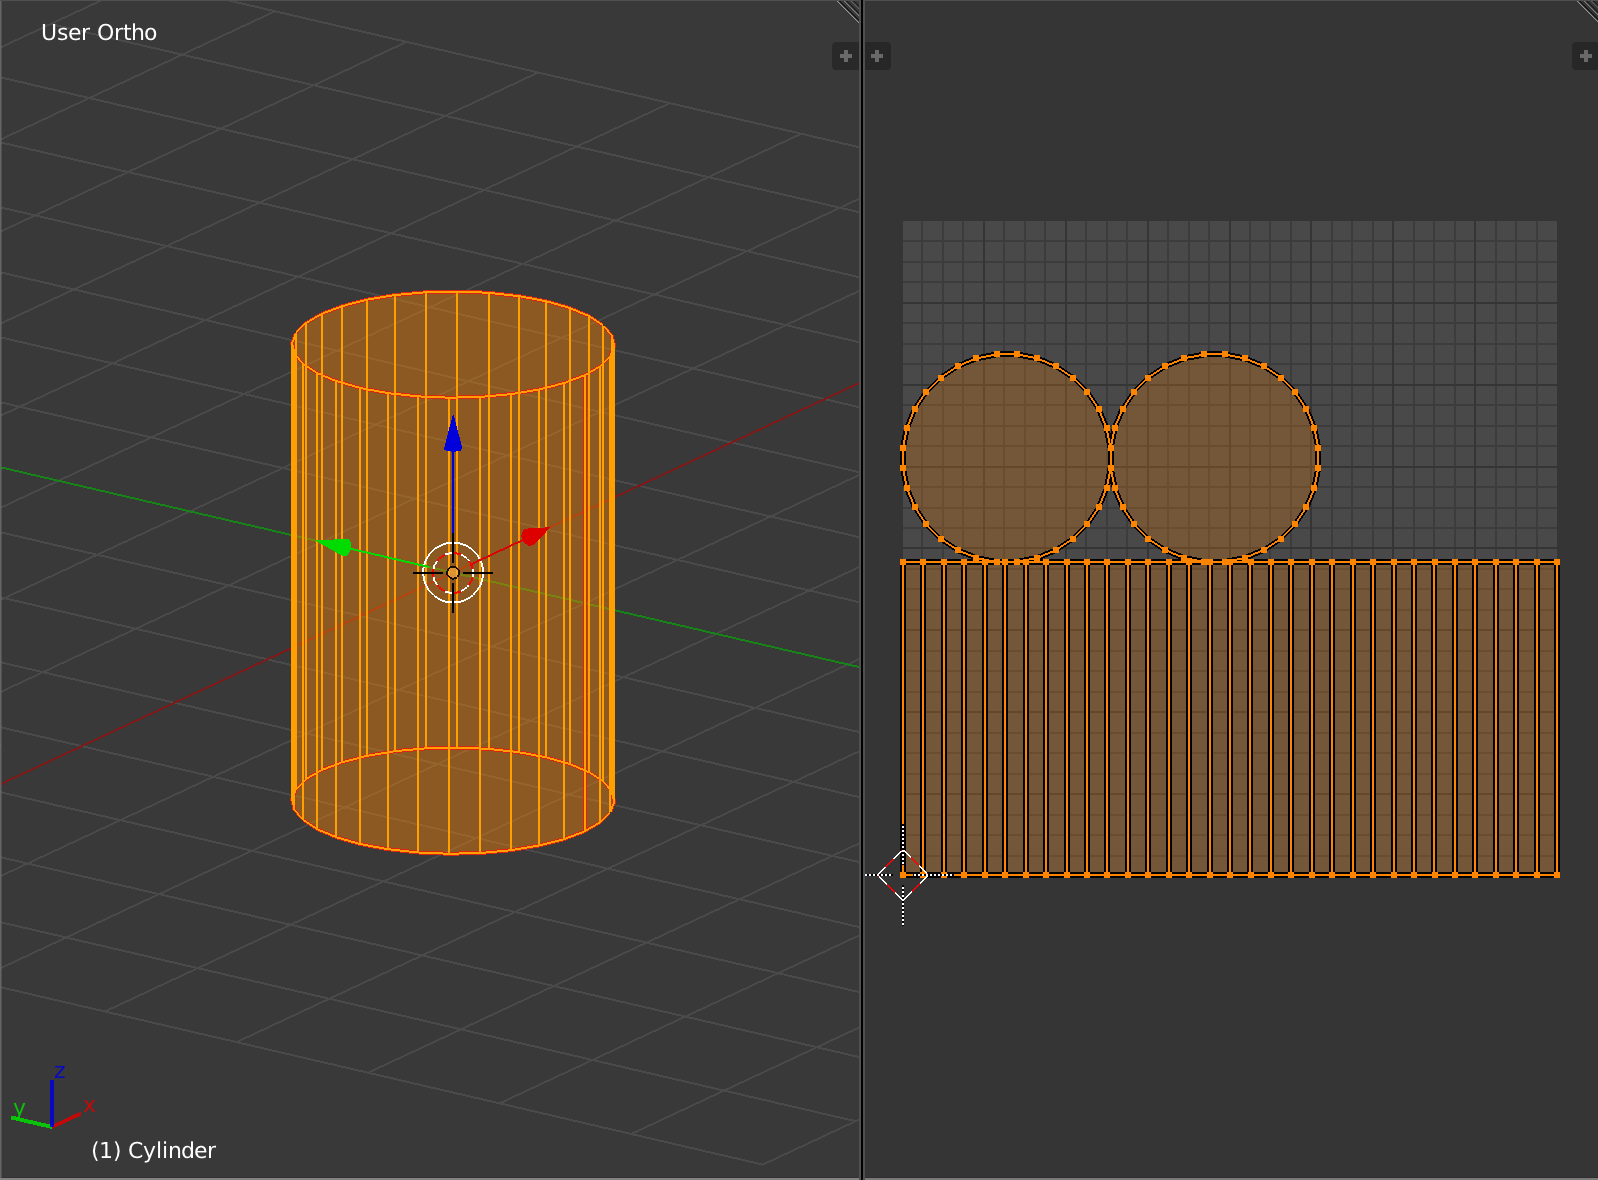
\includegraphics[height=15em]{unwrap-2}}
\end{center}
You can click the 
\includegraphics[height=1.5em]{uvsync-button} button at the bottom of the UV/Image
editor to allow you to select vertices / edges / faces in 2D.  Just like always, you can use 
\keys{G}, \keys{R}, and \keys{S} to transform each face in UV space.  \underline{Select all faces} in the
UV/Image Editor by hovering your mouse over it and pressing \keys{A}, and then navigate to
\menu{UVs>Export UV Layout} at the bottom of the editor.  This allows you to save the UV layout as a
PNG file.  We can now use this as a reference in a standard 2D image editor, like Photoshop or GIMP.

I'll leave creating the texture as an exercise for you.  When the texture has been created, enter
edit mode again and select all faces on the model (\keys{A}).  Then open the texture via the ``Open''
menu at the bottom of the UV/Image editor (
\includegraphics[height=1.5em]{open-texture-button}).
Once again, \underline{make sure all faces on the model are selected} before applying the texture,
and \underline{make sure you are in edit mode}.  Otherwise the texture may not actually apply to the model.
Next change the ``Render Mode'' of the 3D View to \menu{Texture} via a dropdown at the bottom.
Here's what I managed to come up with:
\begin{center}
    \raisebox{-.45\height}{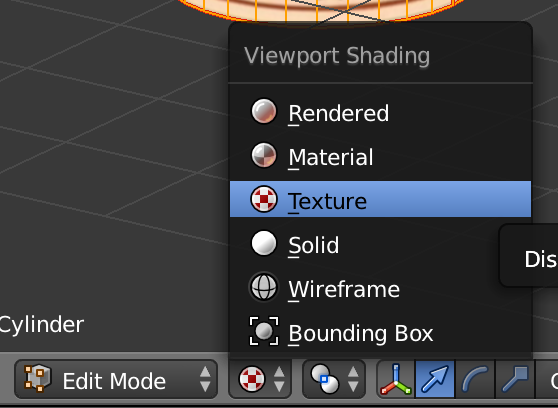
\includegraphics[height=10em]{texture-render-mode}} $\rightarrow$
    \raisebox{-.45\height}{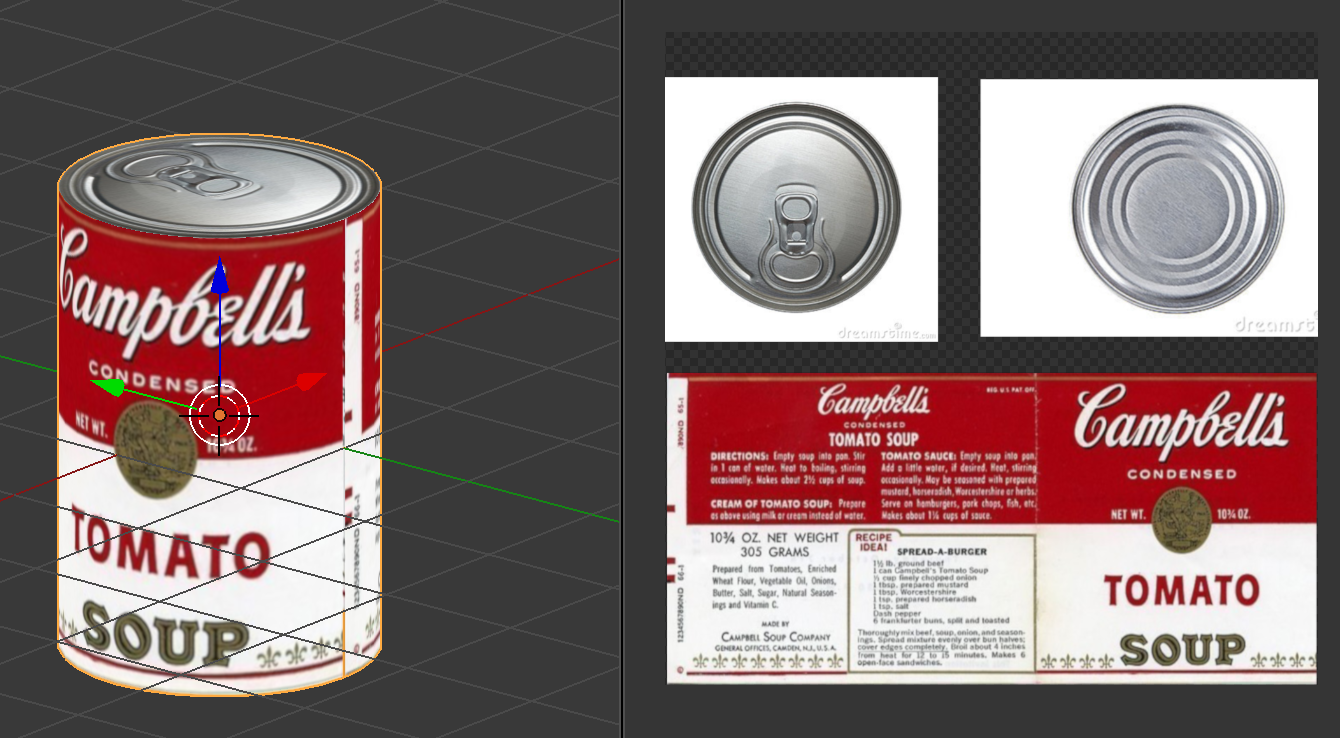
\includegraphics[height=15em]{soupcan-finished}}
\end{center}

\subsection{UV Mapping Complex Models}

UV Mapping is a very complicated topic, and many people build their careers around being great at 
making these textures / maps.  Below I've included where the seams might be placed in the Suzanne
model.  Generally, you want to put the seams in places where it isn't a big deal to see 
discontinuities in the texture.  Good candidates include behind the ears, in the back of the head,
and so on.  You also want to minimize stretching, so you should pick your UV ``islands'' such that
they are easy to unwrap.  One way of ``debugging'' your UV maps is to use a UV test texture.  You
can find plenty of these with a simple Google image search for ``UV Test Texture''.

\begin{center}
    \vbox{
    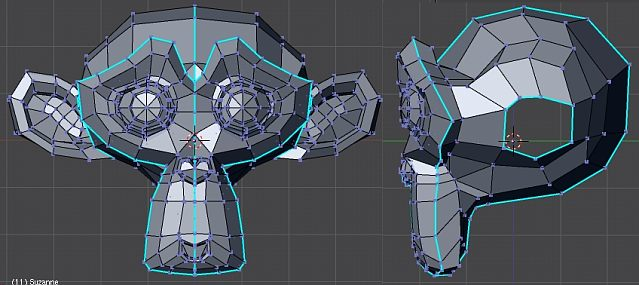
\includegraphics[width=0.75\textwidth]{suzie-seams}\\
    One way of configuring Suzanne's Seams--Source: Blender documentation (\href{https://docs.blender.org/api/htmlI/x5336.html}{https://docs.blender.org/api/htmlI/x5336.html}).}
    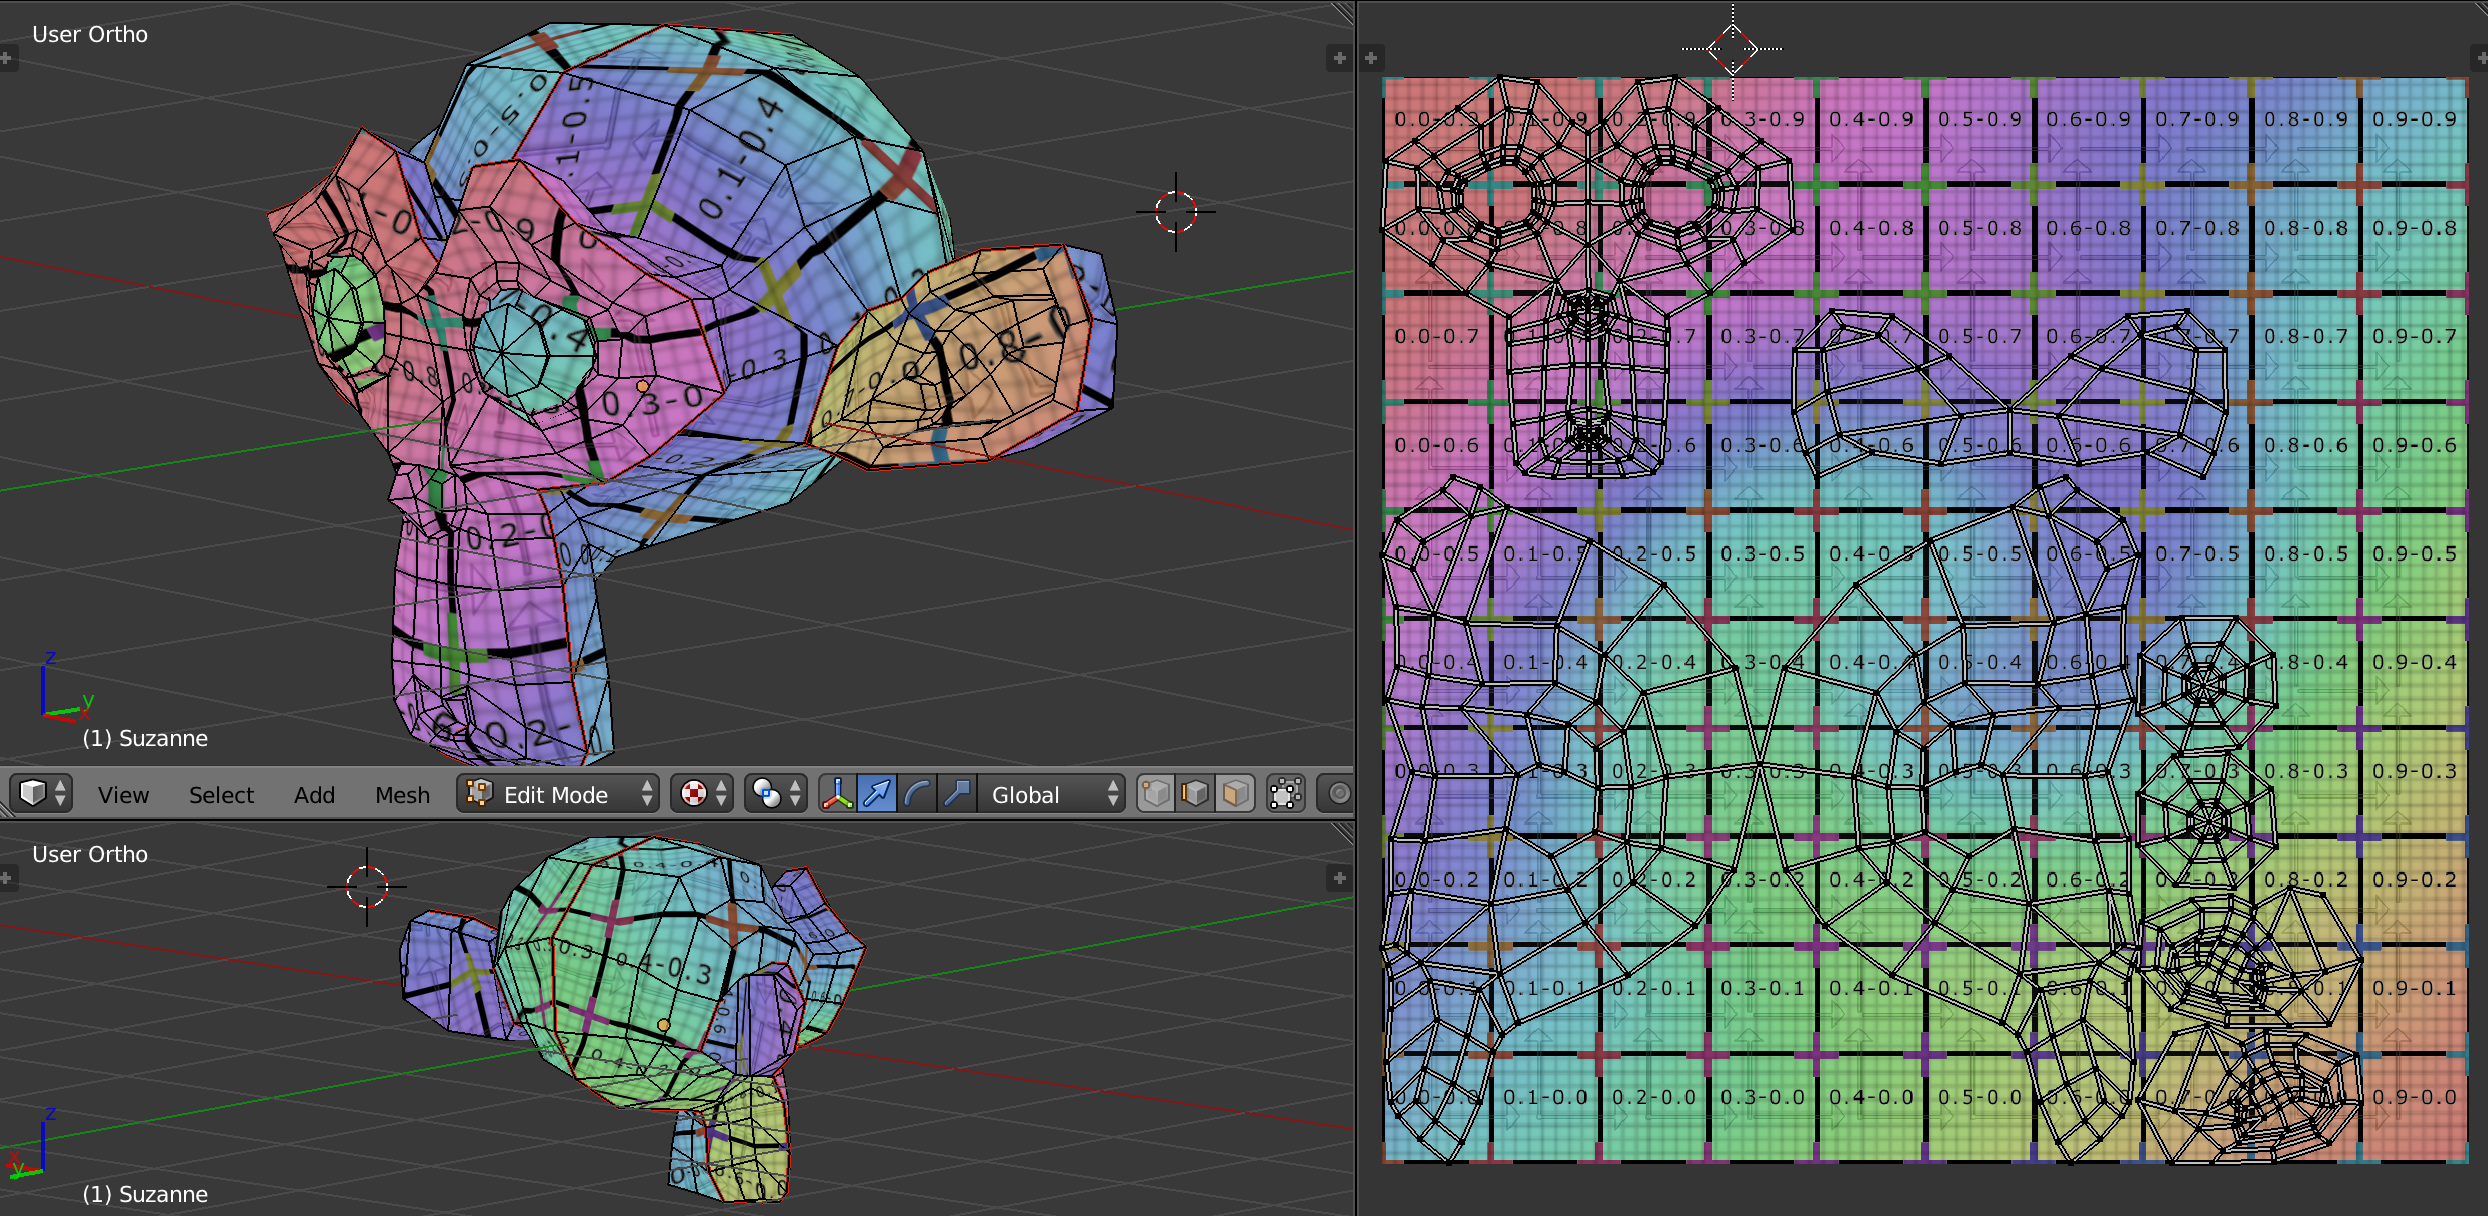
\includegraphics[width=1.0\textwidth]{suzie-textured}\\
    Unwrapping Suzie and applying a UV Test texture
\end{center}

\section{Exporting to Unity}

Unity's native format for 3D Models is \lstinline|.fbx|.  This means that, without any extra software
installed, Unity can load .FBX files by simply placing them in the \directory{Assets} folder.
Unity can also import \lstinline|.blend| files (the blender file format), but you have to have
blender installed to successfully import them.  Similarly, you need to have Maya installed to import
\lstinline|.ma| or \lstinline|.mb| files.  For this reason, I recommend that you always export your
models in blender to .fbx format before importing them into Unity.

You can do this via the menu \menu{File>Export>FBX (.fbx)} at the top of the screen.  You can
configure the export settings on the left side of the file explorer that pops up:
\begin{center}
    \raisebox{-.45\height}{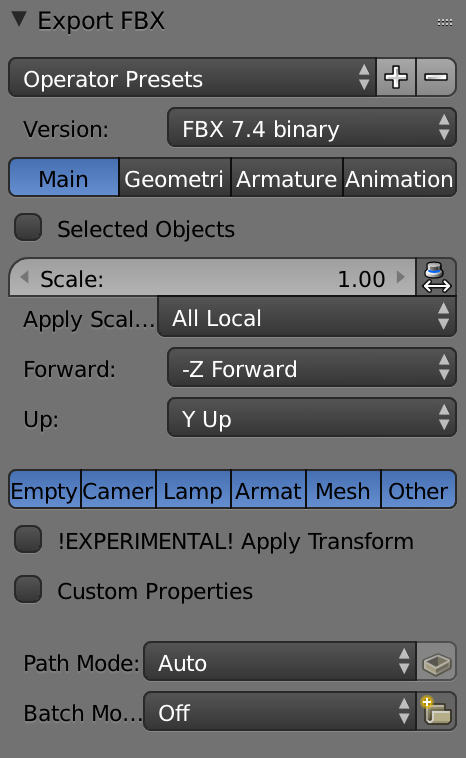
\includegraphics[height=15em]{fbx-export-settings}}\\
    FBX Export Settings
\end{center}
More info on these settings can be found 
\href{https://digitalrune.github.io/DigitalRune-Documentation/html/6f749972-9cb2-4274-b283-c327ba45e379.htm}{at this guide here}.
You can now simply drag the created FBX file into the Project view in Unity.  You will also need to
import whatever textures you have created and apply them to a 
\href{https://docs.unity3d.com/Manual/Materials.html}{Unity material} (more on this in a later lecture).

\section{Exercise}

The exercise for this class is to \textbf{Model, UV, and texture a container} (What is a container?
Up to you$\dots$).  Export the model and import it into Unity!


\end{document}